\documentclass[10pt,twocolumn,letterpaper]{article}

\usepackage{cvm}
\usepackage{times}
\usepackage{epsfig}
\usepackage{graphicx}
\usepackage{amsmath}
\usepackage{amssymb}

% Include other packages here, before hyperref.

%\usepackage[latin1]{inputenc} % Windows
\usepackage[utf8x]{inputenc} % Linux (unicode package needed)
% \usepackage[applemac]{inputenc} % Mac

\usepackage{balance}

\usepackage{graphicx}
\usepackage{caption}
\usepackage{subcaption}

\usepackage{listings}
\usepackage{xcolor}
\usepackage{enumitem}



\colorlet{punct}{red!60!black}
\definecolor{background}{HTML}{FEFEFE}
\definecolor{delim}{RGB}{20,105,176}
\colorlet{numb}{magenta!60!black}

\lstdefinelanguage{json}{
    basicstyle=\scriptsize\ttfamily,
    % numbers=left,
    % numberstyle=\scriptsize,
    % stepnumber=1,
    % numbersep=8pt,
    % showstringspaces=false,
    % breaklines=true,
    % frame=lines,
    backgroundcolor=\color{background},
    literate=
     *{0}{{{\color{numb}0}}}{1}
      {1}{{{\color{numb}1}}}{1}
      {2}{{{\color{numb}2}}}{1}
      {3}{{{\color{numb}3}}}{1}
      {4}{{{\color{numb}4}}}{1}
      {5}{{{\color{numb}5}}}{1}
      {6}{{{\color{numb}6}}}{1}
      {7}{{{\color{numb}7}}}{1}
      {8}{{{\color{numb}8}}}{1}
      {9}{{{\color{numb}9}}}{1}
      {:}{{{\color{punct}{:}}}}{1}
      {,}{{{\color{punct}{,}}}}{1}
      {\{}{{{\color{delim}{\{}}}}{1}
      {\}}{{{\color{delim}{\}}}}}{1}
      {[}{{{\color{delim}{[}}}}{1}
      {]}{{{\color{delim}{]}}}}{1},
}


% If you comment hyperref and then uncomment it, you should delete
% egpaper.aux before re-running latex.  (Or just hit 'q' on the first latex
% run, let it finish, and you should be clear).
\usepackage[pagebackref=true,breaklinks=true,letterpaper=true,colorlinks,bookmarks=false]{hyperref}


 \cvmfinalcopy % *** Uncomment this line for the final submission

\def\cvmPaperID{****} % *** Enter the cvm Paper ID here
\def\httilde{\mbox{\tt\raisebox{-.5ex}{\symbol{126}}}}

% Pages are numbered in submission mode, and unnumbered in camera-ready
\ifcvmfinal\pagestyle{empty}\fi
\begin{document}

%%%%%%%%% TITLE
\title{Computational tools and file format for virtual interactive indoor mapping}

% \author{Marco Virgadamo\\
% Dipartimento di Ingegneria\\
% Universit\`a Roma Tre\\
% Rome, Italy\\
% {\tt\small virgadamo@dia.uniroma3.it}
% Marco Sportillo\\
% Dipartimento di Ingegneria\\
% Universit\`a Roma Tre\\
% Rome, Italy\\
% {\tt\small sportillo@dia.uniroma3.it}
% Federico Spini\\
% Dipartimento di Ingegneria\\
% Universit\`a Roma Tre\\
% Rome, Italy\\
% {\tt\small spini@dia.uniroma3.it}
% \and
% Alberto Paoluzzi\\
% Dipartimento di Matematica e Fisica\\
% Universit\`a Roma Tre\\
% Rome, Italy\\
% {\tt\small paoluzzi@dia.uniroma3.it}
% Antonio Bottaro\\
% Sogei S.p.A.\\
% Ricerca e Sviluppo\\
% Rome, Italy\\
% {\tt\small abottaro@sogei.it}
% }

\author{M. Virgadamo$^1$, M. Sportillo$^1$, F. Spini$^1$, A. Paoluzzi$^2$, E. Marino$^1$, A. Bottaro$^3$ \\[0.5mm]
{\small $^1$Dipartimento di Ingegneria, Universit\`a Roma Tre, Rome, Italy,}  \\
{\small $^2$Dipartimento di Matematica e Fisica, Universit\`a Roma Tre, Rome, Italy,}  \\
{\small $^3$Sogei S.p.A., Ricerca e Sviluppo, Rome, Italy,} 
}

\maketitle
% \thispagestyle{empty}

%%%%%%%%% ABSTRACT
\begin{abstract}

This paper\footnote{This work was partially
supported by grant 2014/15 from Sogei S.p.A., the ICT company of the Italian Ministry of Economy and Finance.} introduces \textsc{\large five} (Framework for Indoor Virtual Environments) and \textsc{\large hijson} (Hierarchical Interactive JSON), respectively a web toolkit for indoor mapping applications and a novel cartographic document format. \textsc{\large five} applications are entirely based on web technologies and rely on \textsc{\large hijson} documents which are in turn processed by a specialized software toolkit. An operative workflow for automated HIJSON documents production using the \textsc{\large lar} representation scheme for topology and geometry, is also outlined.

An \emph{interactive indoor mapping} environment is a virtual reconstruction of a physical indoor space, where the user may interact with virtual objects, experienced in the actual position they occupy in the real world. Our approach outlines a specialized and evoluted  3D \emph{user interface} giving a glimpse of a section of the real world, that the user can handle intuitively.  Furthermore, the virtual indoor environment API provides a platform where many different applications can rely upon. Accessible via web browsers from any kind of device, several applications may coexist on this platform. IoT monitoring, realtime multi-person tracking, and  cross-storey user navigation, are already implemented using an automatic search for all valid walkable routes, and taking into account both architectural obstacles and furniture.

The \textsc{\large hijson} format is used to represent any geometry of the indoor space of complex buildings, capturing their hierarchical structure, a complete representation of their topology, and all the objects (either ``smart'' or not) contained inside. Such textual representation allows the \textsc{\large five} framework to offer a web environment in which the user is presented with 2D or 3D models to navigate. With respect to current cartographic formats, \textsc{\large hijson} introduces four major enhancements: (a) exposes a hierarchical structure; (b) uses local metric coordinate systems; (c) may import external geometric models; (d) accepts semantic extensions.
These semantic extensions encapsulate the details about communication protocols, rendering style, and exchanged and displayed information, allowing the  format to be extended with any sort of models of objects, sensors or behaviors.

\end{abstract}


%%%%%%%%% BODY TEXT

%%%%%%%%% BODY TEXT

\section{Introduction}\label{introduction}

An \emph{interactive indoor mapping} environment consists of a virtual reconstruction
of a physical indoor space, in which the user can move around and interact
with virtual objects, that are found in the same position they actually occupy in the
real world. Such an interactive indoor mapping can be thought as a specialized
and very evoluted \emph{user interface} capable of giving a glimpse of a section of
the real world that the user can handle in a natural and intuitive way. Such
a reconstructed virtual indoor environment can be considered a general
platform where many different applications can rely upon. Both promising and
already well explored ICT applications may find in \emph{virtual indoor mapping} the
perfect context to be integrated into.

In particular, for environments with massive presence of sensor-equipped (or
``smart'') objects, which realize the so-called \emph{IoT} (Internet of
Things), the interactive indoor mapping represents an ideal integrated
interface for IoT monitoring systems. To be specific, it can be the container
of indoor navigation systems, giving the user, to be routed across an indoor
environment, the opportunity to interact with objects along the suggested
paths. Furthermore, in conjunction with the advancements in the field of user
indoor location, whose efforts are nowadays focused to realize an integration
of positioning systems like GNSS (Global Navigation Satellite system), Wi-Fi,
Bluetooth and LTE (Long Term Evolution), to support continuos outdoor/indoor
navigation by means of integration of technologies, it represents the most
natural interface to perform realtime access monitoring and multi-person
tracking. This kind of evoluted user interface is provided by the \emph{FIVE}
Web Framework, whose design choice and implementation details represent the
main contribution of this paper.

To enable such an interactive mapping platform it is of the utmost importance
to set up  a descriptive representation of the indoor environment. A
remarkable contribution of this work is also the definition of the HIJSON
document format, which provides exactly this required descriptive
representation. This description belongs to  the field of indoor cartography,
which as digital evolution of plain floor plans, has arrived to arouse the
interest of big players like Google, that has integrated indoor plans of
specific locations of interest \cite{indoormaps} into Google Maps. In general,
it can be considered ``of interest'' --- such to justify and motivate indoor
cartographic applications --- both public or commercial places of vast
dimensions, as for example airports, train stations, shopping malls, and also
private buildings subject to strict access protocols, like warehouses,
logistic centers, data centers, etc.

Moreover this paper quickly outlines the generation of geometric data of a
complex building, to provide both an explicit semantic and a hierarchical
model of indoor spaces. \textsc{\large lar}, a general representation for
geometric and solid modeling is used for this purpose. The generated
\textsc{\large lar} structures are exported to \textsc{\large hijson} format,
extending \textsc{\large geojson} for indoor mapping and the Internet-of-
Things. A convenient way to extend the representation capabilities of IoT
\emph{smart objects} is also mentioned as semantic extensions, that affects
both document format and the web framework, and can be easily collected in a
public repository.

This work, jointly developed by Sogei S.p.A., an ICT company fully owned by
Italian  Ministry of Economy and Finance, and the CVDLAB (Computational Visual
Design Laboratory) of the ``Roma Tre'' University, is inspired by the
necessities of Sogei itself, which runs one of the largest data center of
Europe, so requiring very strict access control policies, which include the
recording and the real-time interaction with man/machine maintenance
scenarios. Support for this interactive framework, where realtime awareness of
the maintainer position inside the data center helps to reduce intervention
times and to increase safety and security, has been chosen as case study of
interactive indoor mapping, based on the proposed indoor cartographic format.


The remainder of this document is organized as follows. In Section~\ref
{related-work} we provide an overview of the state of the art in the field of
indoor document standards and related applications. Section~\ref{framework} is
devoted to present the FIVE Web Framework, focusing on its architecture and
supported applications, while Section~\ref{hijson} introduces the HIJSON
format specifically defined to describe for indoor environments.
Section~\ref{toolkit} reports about the software toolkit developed to handle
the new document format. In Section~\ref{workflow} it is depicted the
operative workflow adopted to realize the mapping of an hospital. Finally,
Section~\ref{conclusions} proposes some conclusive remarks and future
developments.


% \begin{figure}[!h]
%  \centering
%  \begin{subfigure}[b]{\linewidth}
%  \includegraphics[width=\textwidth]{images/minimum-data}
%  \end{subfigure}
% \\
%  \begin{subfigure}[b]{0.48\linewidth}
%  \includegraphics[width=\textwidth]{images/minimum-colors-a}
%  \caption{}
%  \vspace*{4mm}
%  \end{subfigure}
%  ~
%  \begin{subfigure}[b]{0.48\linewidth}
%  \includegraphics[width=\textwidth]{images/minimum-colors-b}
%  \caption{}
%  \vspace*{4mm}
%  \end{subfigure}
% \\
%  \begin{subfigure}[b]{0.74\linewidth}
%  \centering
%  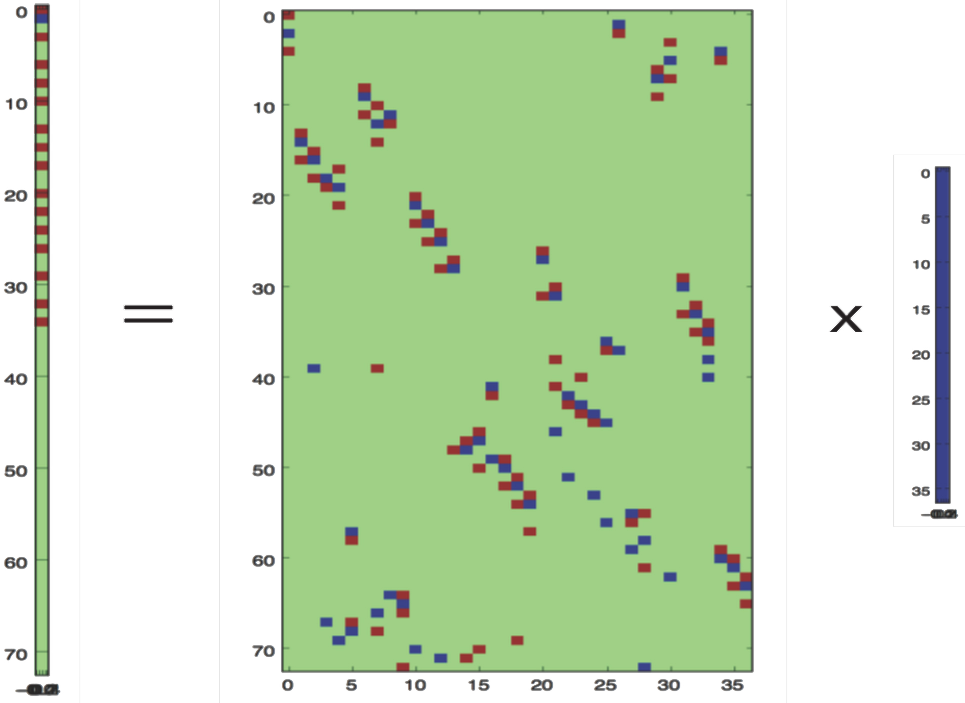
\includegraphics[width=\textwidth]{images/boundary}
%  \caption{}
%  \end{subfigure}
 
%  \caption{A toy example of the LAR scheme: (a) the bare minimum of data with \emph{complete} information about topology; (b) the extracted boundary; (c) the extraction method $[e] = [\partial][f]$ giving the coordinate representation (in the discrete basis of the 1-cells) ofthe boundary edges $[e]$ by product of the sparse boundary operator matrix $[\partial]$ times the coordinate representation $[f]$ of the 2-cells (faces), in the discrete basis of the 2-cells.}
%  \label{fig:minimum-data}
% \end{figure}

% -----------------------------------------------------------------------------


% VASTI AMBIENTI 
% MOLTI SENSORI E SISTEMI DI RILEVAZIONE DELLA POSIZIONE DIFFERENTI
% CONTINUOUS OUTDOOR-INDOOR NAVIGATION
% MONITORAGGIO DI SCENARI UNIFICATI DI INTERVENTO UOMO-MACCHINA
% PERSONALE TECNICO DEVE ESSERE GUIDATO 
% IL PASSAGGIO DA SERVER A IOT È IMMEDIATO
% MONITORAGGIO UNIFICATO DEGLI SMART OBJECTS IOT
% un ambiente indoor virtuale è l'ambiente perfetto per andare a monitorare l'IoT.

% IN QUESTO SCENARIO SI PONE IL LAVORO DESCRITTO IN QUESTO PAPER, 
% IN CUI LE NECESSIT`A DESCRITTE VENGONO AFFRONTATE PARTENDO DALLE BASI,
% OVVERO DEFINENDO UN FORMATO DI DOCUMENTO PER LA DESCRIZIONE ASTRATTA DI AMBIENTI INDOOR.
% DESCRITTO L'AMBIENTE DEVE QUINDI ESSERE POSSIBILE RICOSTRUIRE VIRTUALMENTE L'AMBIENTE
% RENDERLO LARGAMENTE ACCESSIBILE VIA WEB, E MONTARE SU QUESTA RAPPRESENTAZIONE VIRTUALE 
% LA POSSIBILIT`A DI INTERAGIRE CON GLI OGGETTI ALL'INTERNO DELL'AMBIENTE. L'INTERAZIONE DEVE CONSISTERE DA UN LATO NALLA POSSIBILIT`A DI RICEVERE INFORMAZIONI DALL'OGGETTO, MA ANCHE DI INVIARE COMANDI ALL'OGGETTP.

% SI REALIZZA IN QUESTO MODO UNO SCENARIO IN CUI UN SUPERVISORE INTERAGISCE CON L'AMBIENTE IN CUI SI MUOVE UN EXPLORER (O MANUTENTORE) POTENDO IL SUPERVISORE AVERE IMMEDIATA NOTIFICA DELLA POSIZIONE DEL MANUTENTORE, E AVENDO UN QUADRO COMPLETO FORNITO DAGLI OGGETTI SMART PRESENTI NELL'AMBIENTE REALE ASSIEME ALL'EXPLORER.

% D'ALTRA PARTE PER GRANDI SPAZI ANCHE L'EXPLORER PUO ESSERE SUPPORTATO DAL SISTEMA CHE AVENDO COMPLETA CONOSCENZA DELLA TOPOLOGIA E DELLA GEOMETRIA DELL'AMBIENTE, NONCHE DEGLI OGGETTI IN ESSO CONTENUTI, POSSIEDE TUTTE LE INFORMAZIONI NECESSARIE PER GUIDARE L'EXPLORER ATTRAVERSO L'AMBIENTE.

% NULLA IMPEDISCE DI MIXARE LE NECESSITÀ DI EXPLORER E SUPERVISOR, REALIZZANDO UN EXPLORER CHE NAVIGA NELL'AMBIENTE REALE ED IN ESSO RICEVE INFORMAZIONE E A CONTEMPO PUÒ INVIARE COMANDI AGLI SMART OBJECT INTORNO A SE.


\section{Related work}\label{related-work}

The virtual indoor mapping is a youngish field of research resulting from a mix of interdisciplinary knowledge. Thus significative works are not known to the authors at the writing time. Counterwise, research on the cartographic representation of indoor environments is
extensive and heterogeneous with respect to the strategies
applied. Different information sources are used, and accuracy of the
produced solution depends on the adopted approach. In some cases the
information is obtained with automatic or semi-automatic processing of files
that describe the architectural structure of a building, such as BIM (Building Information Modeling)~\cite{Eastman:2008:BHG:1796500} and/or IFC (Industry Foundation Classes) that describe a building project \cite{6816739}. Image processing is also used to
extract topological information from floor plan images \cite{6878152}. In
other works, building information and descriptive parameters are redefined
from scratch \cite{6418876}. Such approaches suffer from the non appropriateness of
their representative formats: images contain poor information and CAD
files are not designed for this kind of use. 

A recurring theme among the use
of cartographic information is \emph{indoor navigation}
\cite{6878152,6418876,6816739}. The proposed approaches are very different in
this case too, and based on several strategies with some basic elements in
common. An often adopted solution is based on the representation of the
routing information as a graph, having a node for each room and an edge for
each pair of connected rooms. In some cases the edges are weighted in
function of Euclidean distance. The detail level of the graph, and hence the
effective usefulness of the calculated paths, can vary depending on the
technique and the design choices applied, but in general most of the proposed
solutions retrieve information only from architectural structure. 

A subject related to navigation is the \emph{location of users}. To locate the exact position of a user inside a
building, the currently most applied techniques are based on fingerprinting and
triangulation of radio signals (Wi-Fi, Bluetooth, LTE, etc.) flanked by more
original solutions based, for example, on image recognition \cite{6815564}.
User tracking issue is faced with solutions that range from the clever
utilization of inertial tracking sensors embedded in many smartphones
\cite{6815564} to the adoption of ad hoc devices \cite{6878152}.

The actual ``de-facto'' standard in terms of geospatial data representation is
the \emph{GeoJSON} format \cite{geojson}, which can be easily used for any type of geographical
annotation. In some cases it has been slightly adapted to be used in indoor
environments: it is the case of the \emph{IndoorJSON} format \cite{indoorjson}.



\begin{figure*}[t!]
\centering
% \includegraphics[width=\textwidth]{images/web_framework_1.png}
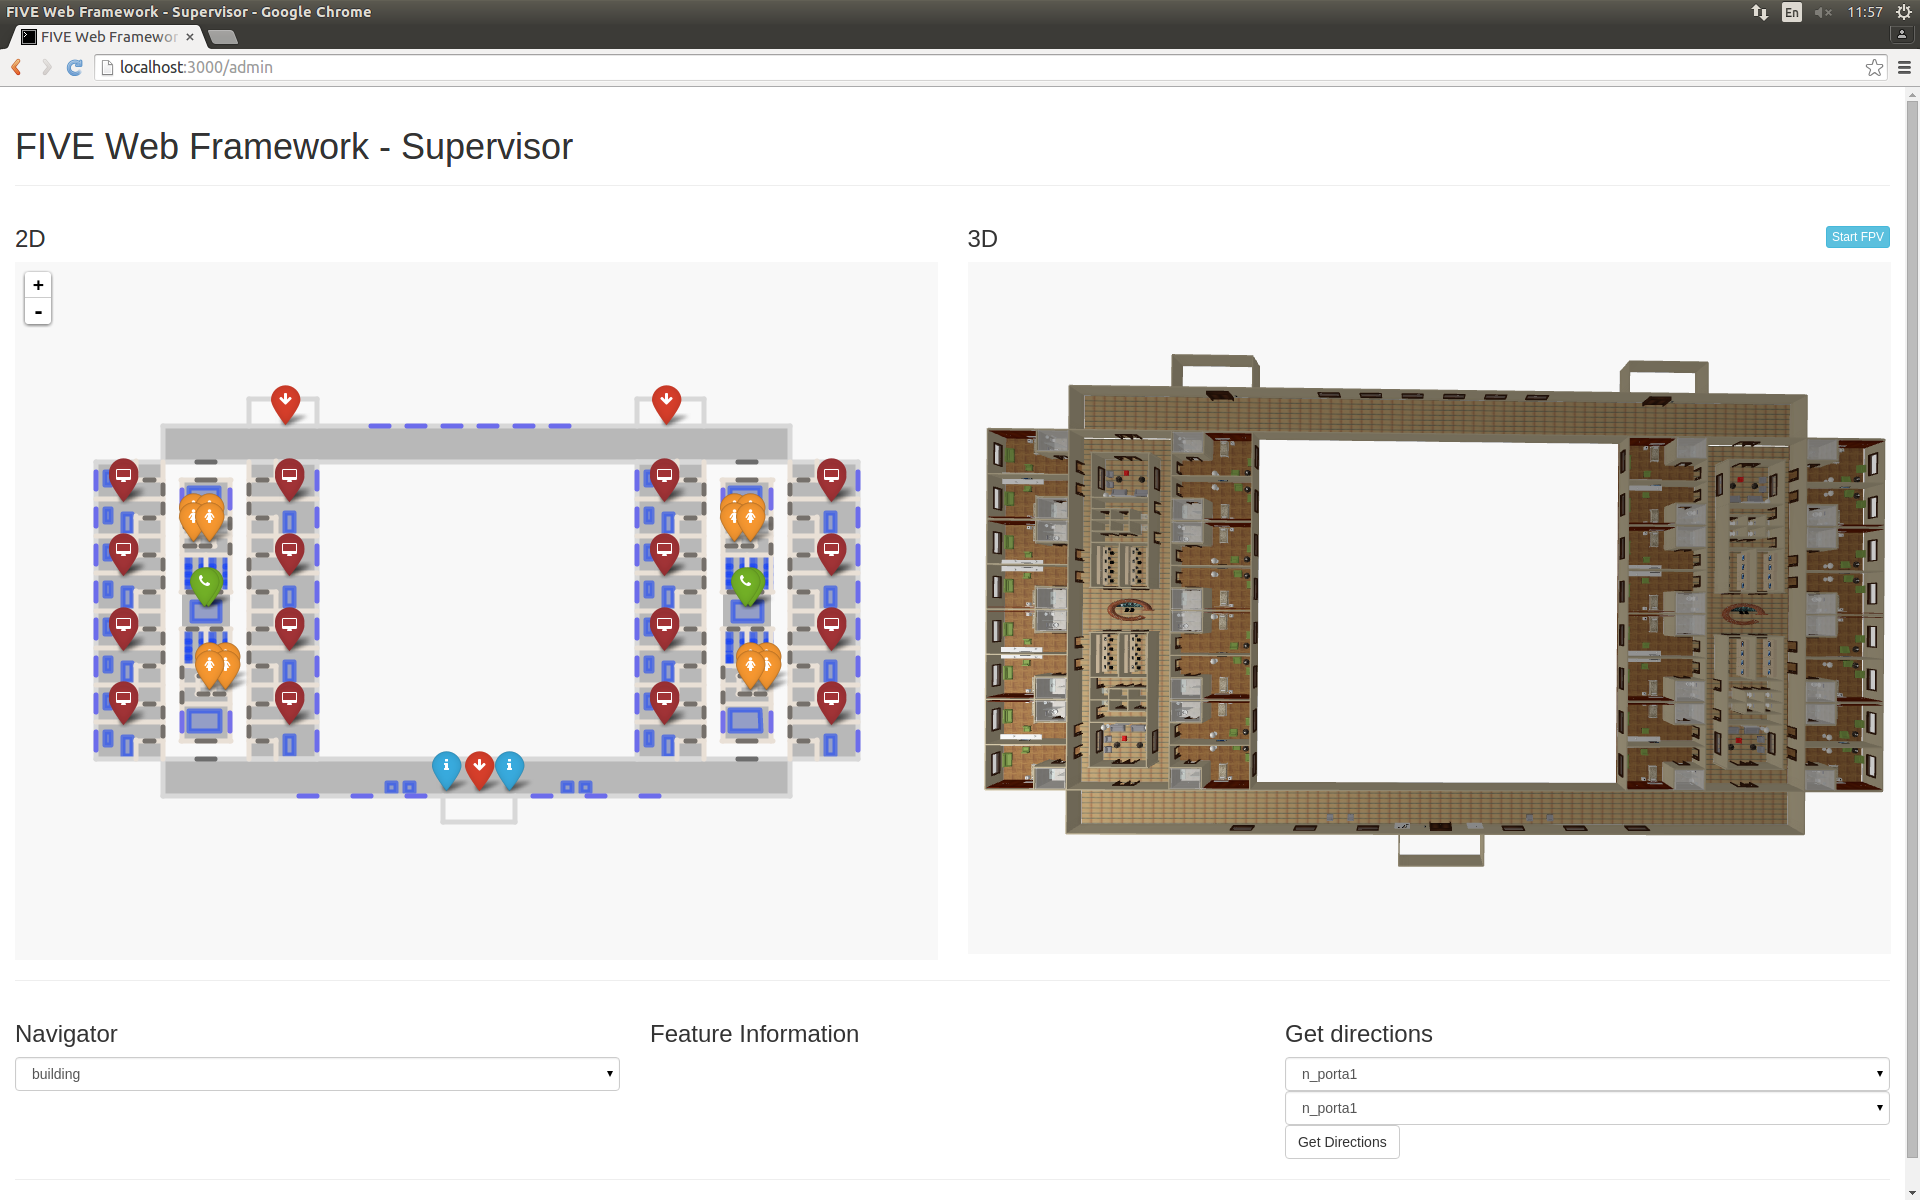
\includegraphics[width=\textwidth]{images/framework-ui.png}
\caption{FIVE Web Framework UI}
\label{fig:web-framework-ui}
\end{figure*}




\emph{GeoJSON} is a geospatial data interchange format based on JSON, suitable for a
geometrical encoding of various geographic data structures. As opposed to GIS
formats, GeoJSON is an open standard. Positions need to be expressed in
geographical coordinates (usually WGS84).

GeoJSON \cite{geojson} allows to define arbitrary objects, called {\tt
Features}, by specifying their {\tt geometry}, and by associtating to them some
{\tt properties}. Complex shapes are defined through the composition of
simple primitive geometric objects. 

Mainly due to its simplicity,
GeoJSON is widely used and deeply integrated into several applications and
services.

\emph{IndoorJSON} \cite{indoorjson} is a GeoJSON variant defined and used by \emph{indoor.io}, a
Finnish company devoted to indoor environment mapping. IndoorJSON is compliant
with GeoJSON syntax, supporting all GeoJSON geometry types.

Customization with respect to GeoJSON format is obtained exploiting particular properties to correctly define the indoor elements: \texttt{level} (which describes which storey contains the feature) and \texttt{geomType} (which identifies the category of the object). A number of non-mandatory indoor properties is also defined: \texttt{accessible} (which describes if an element is walkable or not), \texttt{connector} (which defines if the element is a connection between two
 storeys) \texttt{direction} (which describes the direction of the connection: both
 ways, only up, only down).

A syntax validator is provided by \emph{indoor.io}, but the commercial nature
of this project limits the number of tools available to deal with this
format.


\section{FIVE Web Framework}\label{framework}

FIVE, acronym of \emph{Framework for Indoor mapping in Virtual Environments},
provides a customizable, and scalable web framework realizing an virtual
indoor mapping platform in which multiple applications can convenient resides
on at the same time: IoT,  monitoring, realtime multi-person tracking and
cross-storey user navigation.

Expandability and customizability derive from both design choices and
HIJSON format inherent characteristics, i.e.~the possibility of semantic extensions (see \ref{semantic-extensions}).
Scalability is directly borrowed from technologies used for
software development: \emph{JavaScript} language, using \emph{Node.js},
in particular \emph{Express.js} as backend framework, exploiting the
power of WebSocket protocol through the \emph{Socket.io} library.

Being supported by the \emph{web-as-a-platform}, the framework exposes
also an high availability: it is so simple to use as to visit a
website, both from desktop or mobile devices, without explicit
requirements to install any software package from proprietary stores---access to
which is often denied from business devices.

The FIVE Web Framework deeply relies on HIJSON Toolkit (see \ref{toolkit}) and offers an
all-inclusive client/server architecture with a convenient and highly interactive
user interface, leaving aside the specific indoor positioning system and
the IoT sensors to deal with. A robust application interface is provided and
described in the following section.

\subsection{Applications}\label{applications}

The Framework has been designed with focus on two different kind of
users: the \emph{Explorer} and the \emph{Supervisor}. They have
different requirements and are likely equipped with different devices:
while the \emph{Supervisor} monitors the indoor environment through a
desktop workstation, the \emph{Explorer} has a smartphone available and
needs to be routed across the building.

In both cases, the web platform ensures a perfect alignment with the
BYOD (Bring Your Own Device) approach, nowadays often supported by companies
that encourage employees to use personal devices.


\subsubsection{IoT monitoring}\label{iot-monitoring}

An \emph{IoT monitoring application} consists of an interface showing to the
user, in a single, integrated and centralized way, the information collected
from all the smart objects modelled in the HIJSON document. IoT monitoring
application provides bidirectional communication, since the interface let the
user receive information coming from smart objects while allowing him to send
commands to them.

As the name itself may suggest, it is an activity specifically performed by a
\emph{Supervisor} user, but it can be also suitable to be deployed for the
\emph{Explorer} user, since she can take advantage of the interactive
information coming from the surroundings objects while she moves across the
indoor environment.

Monitoring different smart objects may require different ways to visualize
and/or send data and commands. Modularity and extendibility of the application
respond superbly to these requirements, by providing for each class of objects
a different interface of visualization and interaction, as a result of the
polymorphism principles introduced by the HIJSON Class. In particular, the
user interface is characterized by a dual-display mode, that allows the user
to see at the same time a 2D map that gives an overall glance in a simplified
plan, and a 3D virtual environment to navigate into, as shown in
Figure~\ref{fig:web-framework-ui}.

Alongside with typical smart objects, suitable to deal with like thermostats,
where the user can read the room  temperature and turn the heating on/off,
other kinds of objects, that are not properly considered ``smart'', can be
integrated into the FIVE environment. It is the case, for example, of fire
extinguishers, that are able to show the date of their last check, stored in a
database.

\subsubsection{Realtime multi-person tracking}\label{realtime-multi-person-tracking}

Realtime multi-person tracking allows a \emph{Supervisor} to monitor the
actual position of people inside the building. This kind of task can be useful
for several reasons, including security, logistics or to supervise composite
operative workflows. Each device equipped with the \emph{Explorer} application
is in charge of locating itself, interacting with the indoor positioning
system, and notifying the current position in continuos mode. Evidence of the
people position is given to the \emph{Supervisor} both into a 2D map and an
immersive 3D virtual environment (see Figure~\ref{fig:web-framework-ui}).

\subsubsection{Cross-storey user navigation}\label{cross-storey-user-navigation}

The FIVE Framework also provides the capability to give directions to
\emph{Explorer} users that must move across the indoor environment. The user
specifies a starting and an ending point and the system provides him with a
valid connection path. This feature strongly rely on the graph of paths
generated by the Toolkit (see \ref{automatic-generation-of-valid-paths}), so
starting and ending points must be nodes of the graph. \emph{Connection nodes}
are introduced to represent stairs or elevators, enabling cross-storey paths
to be computed. Since paths can span more than one storey, the most effective
way to display them to the user is to show the connection nodes visualized in
one or more 2D maps.

\subsection{Architecture}\label{architecture}

\begin{figure*}[htb]
\centering
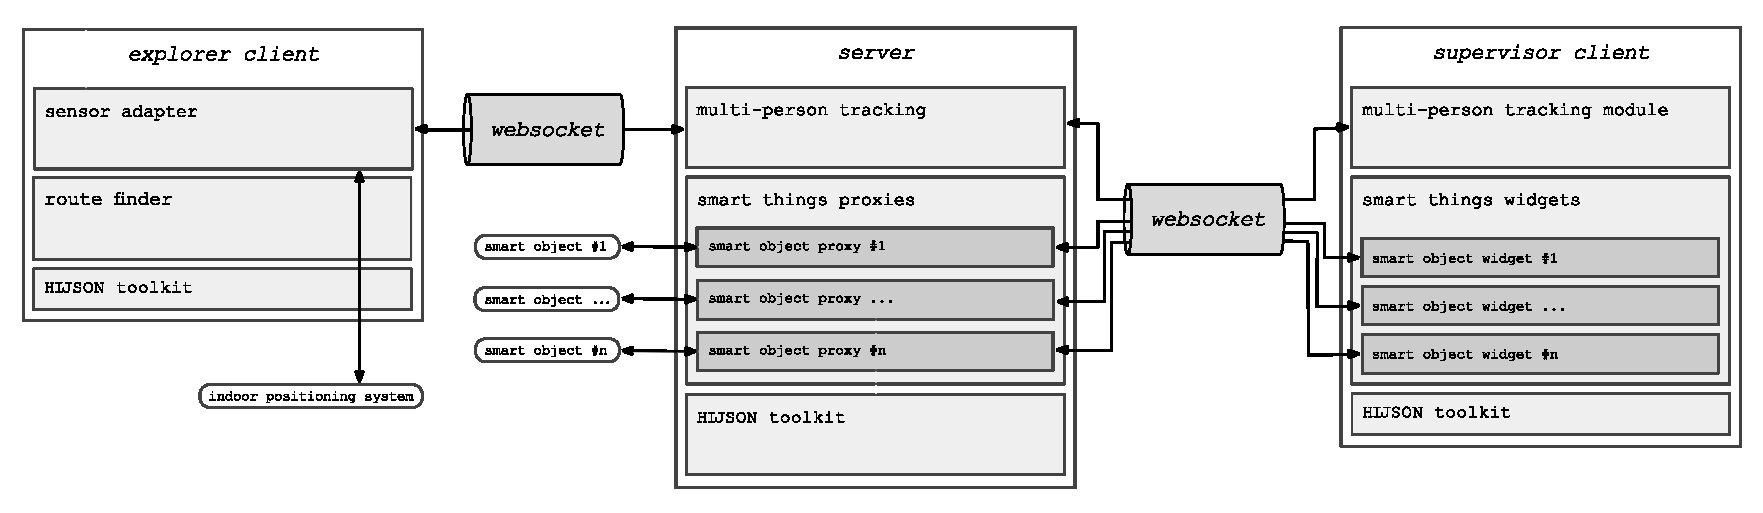
\epsfig{file=images/architecture.eps, width=\textwidth}
\caption{FIVE Web Framework architecture}
\label{fig:architecture}
\end{figure*}

Like the vast majority of the web based applications, the Framework exposes an
overall architecture that is inherently \emph{client/server}. In particular,
two different types of possible clients are identifiable, one for each different 
kind of users: the \emph{Supervisor} client and the \emph{Explorer} client. 
Both of them connect to the same server.

The indoor space described by the input HIJSON document is processed by the
server via the processing pipeline (see \ref{pipeline}). After that, any
connecting \emph{Explorer} client, presumably via a mobile device, will be
provided with the information to perform cross-storey navigation of the
building, while reporting the user position to the server. The server will
feed any connecting \emph{Supervisor} client with users positions, along with
data from sensor-equipped  objects present in the environment, achieving both
IoT monitoring and realtime multi-person tracking.

\subsubsection{Server Architecture}\label{server-architecture}

An architectural scheme of the framework is provided in
Figure~\ref{fig:architecture}. A web server module is responsible for
listening to connecting clients. Each client connection is handled by the web
server module providing all the required resources and then by opening a
WebSocket channel, in order to have both \emph{Explorer} and/or
\emph{Supervisor} communication protocol data flow within. In particular, the
\texttt{multi-person\ tracking} module receives position data from
\emph{Explorer} clients. It aggregates and sends these information to
connected \emph{Supervisor} clients through the WebSocket channel, using a
simple but reliable protocol described later. Independence from particular IoT
sensor equipment communication protocols is achieved introducing a
\texttt{smart\ object\ proxy} module. This one is defined in the HIJSON Class
and is obtained via the \texttt{getProxy()} method (see \ref{hijson-class-definition}) 
for each smart object modelled as described in the follow.

\subsubsection{Explorer client architecture}\label{explorer-client-architecture}

The \emph{Explorer} client architecture is generally deployed on a mobile
device, which is usually supplied to a user who needs to be routed across the indoor mapped
environment. The \texttt{sensor\ adapter} module
encapsulates the communication logic with the indoor positioning system. The
presence of this module ensures independence from particular technologies, so
allowing the \emph{Explorer} client to rely on different indoor positioning
systems (Wi-Fi, Bluetooth, LTE, etc.).

Every time a \texttt{sensor\ adapter} observes a perceptible modification in
user position, it sends the new position information to the server through the
single opened WebSocket, spawning a simple message which includes, beside
current coordinates, the information of the storey of the possibly multilevel
building the user is in.

It is to remark that, when not outflanked by the introduction of an external
server, the problem of communication between positioning system and the low
level APIs of the browser is left to positioning system itself or to whom is
in charge of specific deployments of the FIVE Web Framework.
The \texttt{smart\ object\ widget} module, being in common with the
 \emph{Supervisor} client, will be discussed in the next section.

\subsubsection{Supervisor client architecture}\label{supervisor-client-architecture}

The architecture of \emph{Supervisor} client includes two modules. The first
one, named \texttt{multi-person\ tracking} module, is responsible to
receive through the WebSocket, from the server information about
\emph{explorers} of the environment, showing them in the user interface. The
second module, named \texttt{smart\ object\ widget}, communicates with the
server to propose the user realtime information about sensor-equip\-ped
objects in the environment. Data passes through the single WebSocket
opened between the server and every \emph{Supervisor} client. Relying on a
naive but effective communication protocol, each \texttt{smart object widget}
exchanges data only with its corresponding \texttt{smart object proxy} on the server. To
ensure the data are posted only when the user requires the information
relative to a specific smart object, a \emph{widget lifecycle protocol} is
implemented. This one is based on the four event triggers \texttt{on\_before\_show},
\texttt{on\_show}, \texttt{on\_before\_hide}, \texttt{on\_hide}, as suggested by their names.
When the user requires information about a smart object, its widget has
to be rendered, and \texttt{on\_before\_show} the server is notified to
connect via relative proxy to the sensor. Once connected, the server
begin to send data via WebSocket. Received data are shown through the
widget to the user. When done, the \texttt{on\_before\_hide} event of the
widget is triggered, a notification is sent to the server announcing to stop sending
data, and the proxy closes the connection to the sensor. Widget lifecycle
protocol ensures that only required data are sent from the server to the
client.
 % ex web-framework

\section{The HIJSON format}\label{hijson}

To support the interactive indoor mappong platform, a novel format of
cartographic documents has been defined: it has been named \emph{HIJSON}
(Hierarchical Indoor JSON). It is based upon ideas and design principles
collected from previous formats and identifies four critical improvements with
respect to them: it exposes a \emph{hierarchical structure}, uses \emph{metric
local coordinate system}, may import \emph{external geometric models} and
accepts \emph{semantic extensions}. Furthermore, geometrical  and topological
data can be conveniently imported and represented via LAR (see \ref{lar}), an
advanced representation scheme, allowing to deal with \emph{hyperlinked
geometric models}.



\paragraph*{Hierarchical structure}\label{hierarchical-structure}

The HIJSON format allows for hierarchical description of indoor spaces. The
introduction of a hierarchical structure establishes a parent-child relation
between entities of the model, reflecting a container-contained relationship.
This directly implies a neater representation then the plain linear structure
adopted by GeoJSON, being a perfect analogy of objects contained (i.e.
placed) into spaces.

Therefore, an organized arrangement of spaces is allowed by HIJSON, via
logical (or even physical) grouping: concepts like building wings, sections,
storeys, departments, etc.~can be directly introduced, in order to reflect
into the document structure the actual logical or physical divisions,
categories or relationships among the modelled spaces.

Hierarchical structures are common in computer graphics, where they are used
as scene graphs. This accordance of underlying structures really simplifies 3D
rendering algorithms of HIJSON documented environments. Furthermore, the
container-contained relation enables a recurring use of local reference
frames.

\paragraph*{Metric local coordinate system}\label{metric-local-coordinate-system}

Supported by the hierarchical underlying structure, the HIJSON document format allows 
the use of local coordinate systems. Hence the shape of all elements can 
be conveniently modelled using local coordinates, and then placed in the right position 
with respect to the position of the parent (or container) element applying a rotation, followed by a
translation transformation.

Moreover, the adoption of a metric reference frame simplifies the compilation
of the document, either manually generated or produced by software tools. Just
remember that the GeoJSON coordinates are geographical, a pairs of (absolute)
latitude and longitude angles, like the ones provided by GNSS systems. This
kind of coordinates  are certainly not particularly user friendly, when
positioning a smart device or a furniture element within a specific building
room.

The HIJSON document format is specially designed to guarantee the user to be routed seamlessly 
from outdoor to indoor and vice versa. Even if indoor geometries are entered in a local metric 
coordinate system, continuos outdoor/indoor navigation is ensured through the processing pipeline
detailed below.

\paragraph*{Semantic extensions}\label{semantic-extensions}

Semantic extensions make the HIJSON format extendible and customizable, that
is able to adequately respond to any need of objects representation. To define a
semantic extension means to allow the HIJSON document to model an object
previously not covered, or even to modify the behavior of a comprised one.
Semantic extensions are to be defined both as HIJSON format syntax and as
HIJSON Toolkit source code. In particular it is necessary to define respectively
a new HIJSON Element and a new HIJSON Class, as specified below.

% \paragraph*{Hyperlinked geometric models}\label{hyper-linked-geometric-models}

% The HIJSON document may further import external geometric models --- either of the buildings themselves or the interior furniture or devices --- that are topologically complete (in the sense of solid modeling~\cite{Requicha:1980:RRS:356827.356833}) and very compact. 
% Such models, coming from a source outside the document, are acquired by hyperlinking JSON files that contain a Linear Algebraic Representation (LAR) of topology and geometry, to be expanded for visualization or interaction at any useful level of detail. 

% The LAR scheme~\cite{Dicarlo:2014:TNL:2543138.2543294} is characterised by a very large domain, including architecture, building and construction~\cite{paoluzziMS:2014}, 2D and 3D engineering meshes, non-manifold geometric and solid models and meshes, and high-resolution 3D images~\cite{cadanda:2015}. This scheme uses the set of \emph{Combinatorial Cellular Complexes} (CCC) as mathematical domain
% \cite{Basak:2010}, and various compressed representations of \emph{sparse matrices} \cite{gemmexp} as codomain. 

% Since LAR provides a complete representation of the topology of the represented space,
% the matrix $[\partial_d]$ of the boundary operator shall be used to compute the coordinate representation $[c]$ of the \emph{boundary} chain of \emph{any subset} $c$ of cells, though \emph{a single} operation of SpMV multiplication \cite{gemmexp} between the \texttt{CSR} (Compressed Sparse Row) representation of $[\partial]$ and the \texttt{CSC} (Compressed Sparse Column) representation of the $[c]$ chain, resulting in very efficient computations on modern hardware, even mobile.

% The expansion of a LAR model, to be considered as a general-purpose graphic primitive, may be executed on either the server or the supervisor client of the HIJSON Web Toolkit architecture (see Section~\ref{server-architecture}), or even on the \emph{Explorer} client, depending on the size and the locality of the model to be expanded.

% \begin{figure}[htbp] % figure placement: here, top, bottom, or page
% \centering
% \includegraphics[width=\linewidth]{images/sogei} 
% \caption{Office building: (a) the schematic plan; (b) the simplified 3D model generated for testing on the field the in-door mapping project described in this paper.}
% \label{fig:sogei}
% \end{figure}



\subsection{Structure and syntax}\label{syntax-structure}

A HIJSON document is composed by a configuration section, followed by one or more \texttt{FeatureCollections}, containing the actual data.

Listing~\ref{lst:hijson-example} shows a simplified HIJSON document, devoid of punctual details, to make clear to the reader the overall document structure.

% \vfill

\begin{lstlisting}[language=json, label={lst:hijson-example}, captionpos=b, caption=Example of HIJSON document.]
{
  "config": {
    // ...
  },
  "data": [
    // ...
    {
      "id": "architecture",
      "type": "FeatureCollection",
      "features": [
        // ...
      ] 
    },
    {
      "id": "furniture_1",
      "type": "FeatureCollection",
      "features": [
        // ...
      ] 
    },
    // ...
  ]
}
\end{lstlisting}


The configuration includes parameters and settings needed for building representation in the form of a JSON Object. One of the core information in this section is defined by the correspondence between three points of the local coordinate system and three points of the real world, expressed in geographical coordinates. This is needed to ensure a seamlessly passage from local to geographical coordinate system and vice versa.

After the configuration part, the document includes a list of \texttt{FeatureCollection}. An example
of \texttt{FeatureCollection} is given in listing~\ref{lst:feature-collection-example}.

Each element of the list is given in the form of a GeoJSON {\tt
FeatureCollection}, that contains an arbitrary  number of HIJSON Elements.
Each \texttt{FeatureCollection} imposes a logical relationship that can be used
to group together related HIJSON Elements. Since  HIJSON Elements adhere to
the GeoJSON format, each \texttt{FeatureCollectio}n results compliant with GeoJSON
syntax and then accepted by any GeoJSON validator. As detailed below, the
HIJSON format  introduces some additional rules that allow the adoption of
this format for indoor representation.

\begin{lstlisting}[language=json, label={lst:feature-collection-example}, captionpos=b,  caption=Example of \texttt{FeatureCollection}.]
{
  "id": "architecture",
  "type": "FeatureCollection",
  "features": [
    // ...
    {
      "type": "Feature",
      "id": "room_0.1",
      "geometry": {
        "type": "Polygon",
        "coordinates": [
          [ [0, 0], [11, 0], [11, 19], [0, 19] ]
        ]
      },
      "properties": {
        "class": "room",
        "parent": "level_0",
        "description": "Office of Mr. Smith",
        "tVector": [10, 20, 0],
        "rVector": [0, 0, 90]
      }
    },
    // ...
  ]
}
\end{lstlisting}


\subsubsection{HIJSON Element}

Dealing with indoor environments, there are essentially two classes of objects
that is necessary to represent. They are (a) architectural elements, like a
room, a corridor, a wall, etc. and (b) furnishings, intended in a broad sense,
such as to contain both furniture, like a desk or a chair, and/or ``smart objects'',
like an IP-cam or a connected thermostat.

A HIJSON Element defines a GeoJSON compliant syntax to describe both geometry and properties of
an object. It represents the atomic component of a HIJSON document. 
It would be a best practice to group
together related JSON Elements using \texttt{FeatureCollections}: several classification strategies
can be applied, for example by grouping the elements by storey or even by room.
Alternatively, since the furnishings are more likely to change than the
architectural components of a building, these two different kinds of elements
can be isolated in different \texttt{FeatureCollections}, as it has been done in the listing~\ref{lst:hijson-example}.

The hierarchical structure of the document gives visible form to the capability of HIJSON Elements to have children elements. A unique ID is mandatory for every HIJSON Element. 

Three Geometry types can be used here: \texttt{Point}, \texttt{LineString}  and {\tt
Polygon}. The choice of the Geometry type to be associated to a HIJSON Element
implicitly defines the category of the element: \texttt{Point} is used for
furnishings, \texttt{LineString} for walls and doors, while \texttt{Polygon} may
describe levels and rooms.

The Geometry coordinates are expressed in metres, by convention starting at
the bottom-left corner of the element, whose position is used to set-up the
origin of a local coordinate frame. Unlike GeoJSON, where all properties are
optional, in HIJSON some strict requirements are imposed, and some attributes
are mandatories: a) \texttt{class} (representing the element category, used to
instantiate  the appropriate \emph{HIJSON Class}), b) \texttt{parent}
(containing the ID of the parent of the element), c) d) \texttt{tVector}
(representing the translation relative to   the parent element, expressed in
metres), e) \texttt{rVector} (representing the rotation relative to   the
parent element, expressed in nonagesimal degrees).

Specific classes may require the mandatory presence of other properties. For
example, the classes \texttt{internal\_wall} and \texttt{external\_wall} that
define the internal partitions and the external envelope, respectively, require a \texttt{connections}
array, containing the IDs of the adjacent elements. This information is used
by the connector children of the element (e.g. doors) to identify the
areas linked together.

Given the nature of the GeoJSON format from which HIJSON derives, the elements
are represented by their 2D shape, like on a planimetry. The property {\tt
height} was introduced to assign a value to the height of the object, intended
as a third dimension.

A \texttt{description} property can provide further information about
the element.
Arbitrary optional fields can be added without restrictions, in order to
enrich and extend the expressivity of the representation, or simply for the sake of 
documentation.
 % ex advances and syntax

% \vfill


\section{HIJSON Toolkit}\label{toolkit}

The HIJSON Toolkit is a software module that implements common operations and
transformations on HIJSON documents. Written in \emph{JavaScript} language,
this software module has been built to be deployed in the web environment. It
is \emph{modular} and entirely \emph{isomorphic}, i.e.~can run on the server
as well as on every client. It relies on libraries and frameworks such as
\emph{React}, ``the JavaScript library for building user interfaces'' by
Facebook, and as \emph{Three.js}, the current de-facto standard to deal with
\emph{WebGL} technologies.

The Toolkit executes the instantiation and extension logic of a HIJSON
document, and provides a multistage transformation pipeline that, according to
the requirements, can be used either entirely or only in part.

\subsection{Processing pipeline}\label{pipeline}

The HIJSON processing pipeline implements the sequence of preliminary
transformations that have to be applied to a HIJSON document before any
further operation. It is not strictly required to complete each stage of
the pipeline: the exit stage depends on the specific use case.

The application of the transformation pipeline has a double aim. The first one
consists in generating the graph of valid paths among all the interesting
elements. The second objective is the generation of one \emph{GeoJSON}
document for each storey of the building described by the HIJSON document. In
this way a bidimensional layout  can be provided for every level of the building, 
and visualized through any compliant GeoJSON viewer.

The HIJSON processing pipeline is composed by six elaboration stages, denoted
as \emph{validation}, \emph{georeferencing}, \emph{parsing}, \emph{graph paths
generation}, \emph{2D layers generation}, \emph{marshalling}. The pipeline of
transformations and the output of each stage are shown in
Figure~\ref{fig:pipeline}.

\begin{figure}[!htbp]
\centering
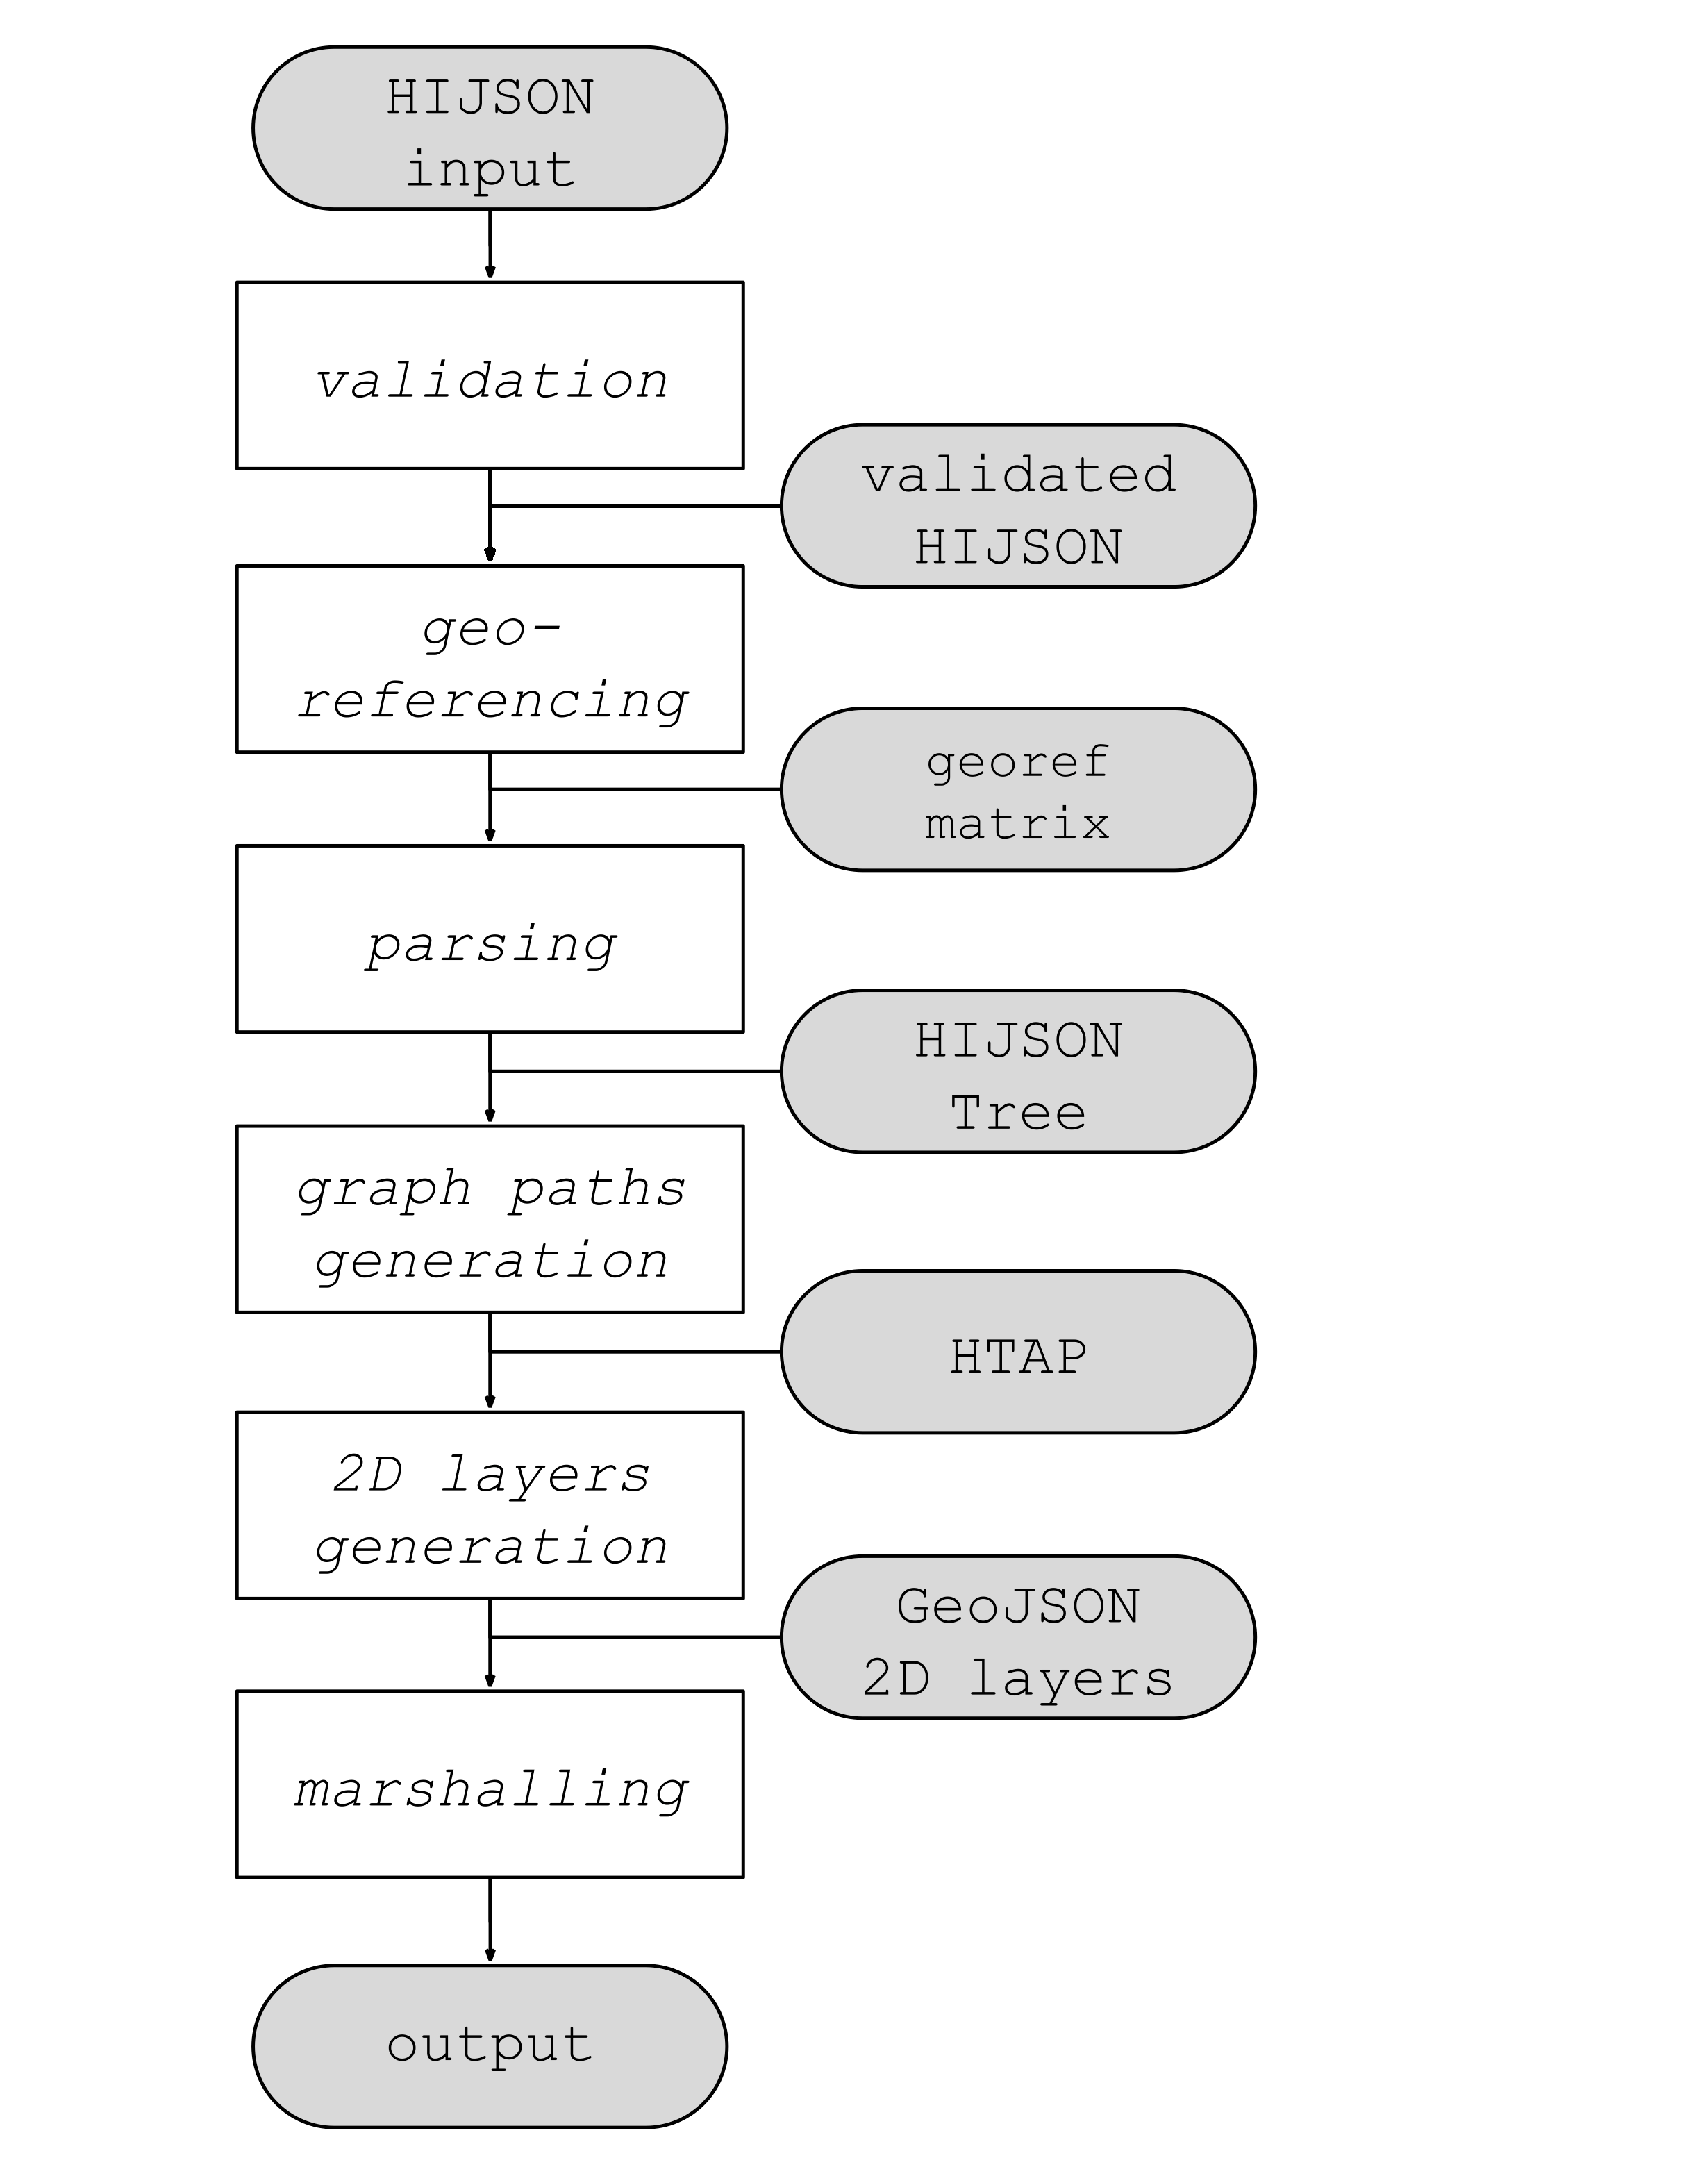
\epsfig{file=images/pipeline.eps, height=0.4\textwidth}
\caption{HIJSON processing pipeline}
\label{fig:pipeline}
\end{figure}

% \begin{enumerate}[noitemsep,topsep=0pt,leftmargin=*]
% \item
 1. \textit{\texttt{validation}} - The first one is the validation stage. In
  order to begin with the effective transformations the input HIJSON  document
  must be compliant with both the syntax format and the structural requirements.   In the
  case the validation stage fails, processing aborts and does not continue to
  following stages; intead if this stage successes, then the output for the next stage is a
  validated  HIJSON.

% \item
 2. \textit{\texttt{georeferencing}} - In the second stage, in order to allow
 for continuous outdoor/indoor navigation, the system needs to compute
 the georeferencing matrix, a linear operator able to transform local
 coordinates into global coordinates (world coordinate
 system --- latitude and longitude angles) and vice versa. This task is
 accomplished by solving a linear system obtained from information
 contained in HIJSON configuration part and precisely from the
 correspondence of three real world points to three points included
 into the HIJSON document.

% \item
 3. \textit{\texttt{parsing}} - The parsing stage takes the validated and
 georeferenced HIJSON as its input, that as illustrated before can be
 thought of as a list of HIJSON Elements, parses them and produces an
 instance of the HIJSON Tree. The HIJSON Tree is an object in memory
 representing the hierarchical structure of the building described
 by the HIJSON document.

% \item  
 4. \textit{\texttt{graph of paths generation}} - The fourth stage is
 in charge  of the generation of the graph of paths 
 (see \ref{automatic-generation-of-valid-paths}). The graph of paths can
 be used to compute valid directions between pairs of points of  interest
 inside the building model. Once the graph of paths has been computed, the
 input HIJSON Tree is augmented with paths information, becoming what  has been
 called an HTAP (HIJSON Tree Augmented with Paths).  Augmentation always takes
 place in the form of an addition of leaf nodes as children of a  specific
 element (e.g. ``room'').

% \item
 5. \textit{\texttt{2D layers generation}} - The fifth stage concerns the
 generation of GeoJSON \emph{layers}. For each storey of the building, the Toolkit generates a
 GeoJSON layer that can be used for the creation of a 2D map. Each layer
 contains only the children of a `level' node of the HIJSON Tree. 
 The presence of a specific element inside the layer can be finely tuned 
 by means of a Boolean value. The geographical coordinates of every elements
 are calculated by a series of multiplications between transformation matrices obtained 
 during the tree traversal to the local coordinates.

% \item
 6. \textit{\texttt{marshalling}} - The last stage is responsible for executing
 a serialization of the the transformed data. This stage, in which are performed tasks like breaking
 dependency-loops and stringification, is
 mainly useful  server-side, as the output is there stored ready to be
 served to any requiring client.
% \end{enumerate}

\subsubsection{Automatic generation of valid paths}\label{automatic-generation-of-valid-paths}

The fourth stage of the processing pipeline is responsible for the
generation of a graph of valid paths through the entire model
represented by the input HIJSON document. The graph generated according
to the algorithm described in the following, although non optimal,
ensures a complete coverage of the surface while limiting the number of
generated nodes. The resulting graph is weighted on the edges with nodes
distances. Each graph node may represent either: a) a \emph{standard path node}, i.e.~a junction node or possibly an endpoint of a path; b) a \emph{connection node}, used as subproblem composing element in the divide et impera approach adopted; c) an \emph{element node} i.e.~HIJSON Element (whose HIJSON Class explicitly grants his presence in the graph), typically an endpoint of a path.

The graph of paths allows for calculations of directions between any two given
nodes. Although different approaches have been explored \cite{6999103}, 
a very classical solution has been selected in this case, so directions 
are actually computed client-side by applying the Dijkstra algorithm to the graph. 

Taking advantage of the hierarchical structure of the HIJSON document,
and according to the divide et impera approach, the problem of 
paths generation is split in several sub-problems, which consist in
the computation of the sub-graphs relative to each individual space, more generally a single room. The sub-graphs are then linked together through the
connection nodes (which in most cases represent doors). The resolution
of each sub-problem (as depicted in Figure~\ref{fig:graph-generation}), 
is composed by four steps. 

1. \textit{Computation of the walkable area of the space}: this task is
 accomplished by subtracting the shape of the obstacles from the area
 of the space; the result is typically a surface with holes.

2. \textit{Triangulation of the walkable area}: the computed surface is
 triangulated taking into account the presence of holes.

3. \textit{Identification of graph nodes}: for each triangle side completely
 internal to the area, its midpoint is selected as standard path node.

4. \textit{Junction of nodes}: nodes relative to the same triangle are then linked
 pairwise; both element nodes and connection nodes (i.e.~doors) are
 linked to the nearest node of the space (i.e.~room).

\begin{figure}[!htbp]
 \centering
 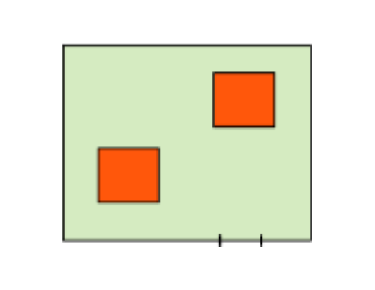
\includegraphics[angle=-90,origin=c,width=.22\linewidth]{images/graph-generation/single/graph-generation-1}
 ~
 
\includegraphics[angle=-90,origin=c,width=.22\linewidth]{images/graph-generation/single/graph-generation-2}
 ~
 
\includegraphics[angle=-90,origin=c,width=.22\linewidth]{images/graph-generation/single/graph-generation-3}
 ~
 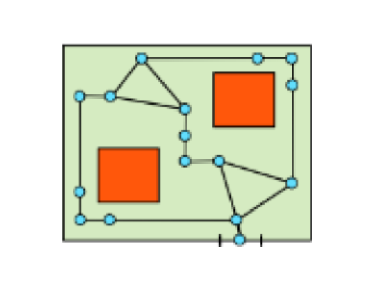
\includegraphics[angle=-90,origin=c,width=.22\linewidth]{images/graph-generation/single/graph-generation-4}

 \caption{the 4 steps graph of paths generation}
 \label{fig:graph-generation}
\end{figure}

\subsection{HIJSON Class definition}\label{hijson-class-definition}

To make better use of the possibilities offered by the HIJSON Toolkit and by the
HIJSON document format, some custom dynamic behaviors can be described. These
behaviors encapsulate the specificities relative to communication
protocols with the sensors, as well as to features of user interaction. The
interface for such behavior is the HIJSON Class.

\begin{figure}[!h]
\centering
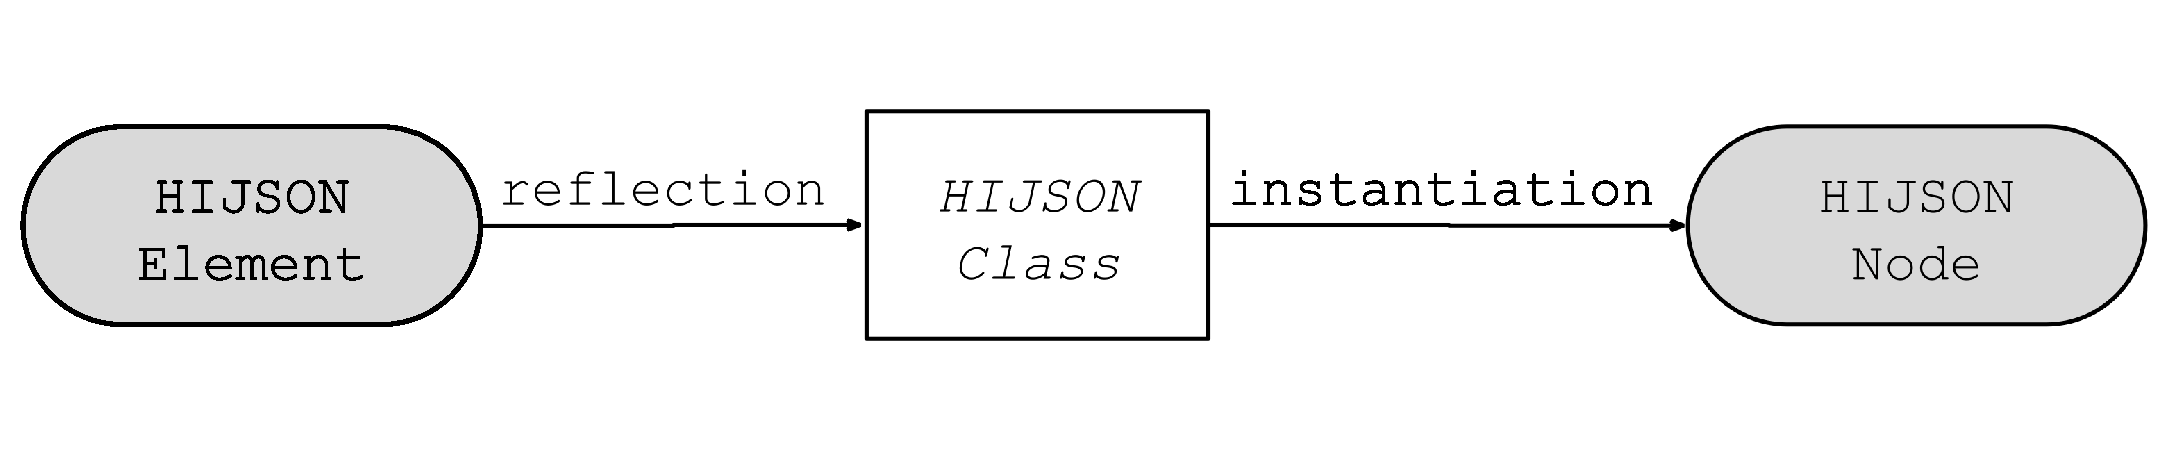
\epsfig{file=images/element-class-node.eps, width=0.44\textwidth}
\caption{HIJSON Element/Class/Node relashionship}
\label{fig:elem-class-node-rel}
\end{figure}

Every HIJSON Element of the input HIJSON document has a dynamic
counterpart, a running instance called \emph{HIJSON Node}, instantiated
according to the corresponding HIJSON Class via reflection methods (see
Figure~\ref{fig:elem-class-node-rel}).

To specify a new \emph{HIJSON Class} means to extend the Toolkit to deal with a
new class of HIJSON Element.
To extend the toolkit in order to deal with a new class of HIJSON Element is
required to specify a new HIJSON Class, by defining the following
properties and methods:

\begin{itemize}[noitemsep,topsep=0pt,parsep=0pt,partopsep=0pt,leftmargin=*]
\item
 \texttt{in\_graph}: a Boolean value to express if the element is an
 approachable point in the graph of paths;
\item
 \texttt{in\_2D\_map}: a Boolean value to express if the element must 
 be shown in the 2D map;
\item
 \texttt{get2DStyle()}: a method that returns the 2D map appearance of
 the element, essentially HTML and CSS code;
\item
 \texttt{get3DModel()}: a method that returns the 3D model appearance of
 the element, i.e.~an instance of \texttt{Obj\-ect\-3D} of the \emph{THREE.js} 
 framework;
\item
 \texttt{getWidget()}: a method that returns the information widget, a
 \emph{React} component;
\item
 \texttt{getProxy()}: a method that returns the server-side proxy which
 encapsulate the IoT sensor communication protocol, i.e.~a \emph{Node.js}
 module.
\end{itemize}

User's needs for new indoor elements, greatly different sensor equipments,
alternative representations of 2D or 3D viewports are accepted by the
definition of new HIJSON Classes, that so provide single-point
custom extensions of the Toolkit capabilities.


\section{Virtual indoor mapping generation workflow}\label{workflow}

The 2.5D model of the built environment to interact with is generated offline and server-side, finally producing a HIJSON format.
Currently, we produce the HIJSON document from a python
script using two libraries for geometric computing (\texttt{pyplasm} and \texttt{larcc} \cite{Dicarlo:2014:TNL:2543138.2543294,paoluzziMS:2014,cadanda:2015}).

The modeling process will be improved by implementing a LAR-based 
graphical editor to assist the user during the description of the indoor
space. The realization of such an editor is already in our plans.


\begin{figure*}[ptb] %  figure placement: here, top, bottom, or page
   \centering
   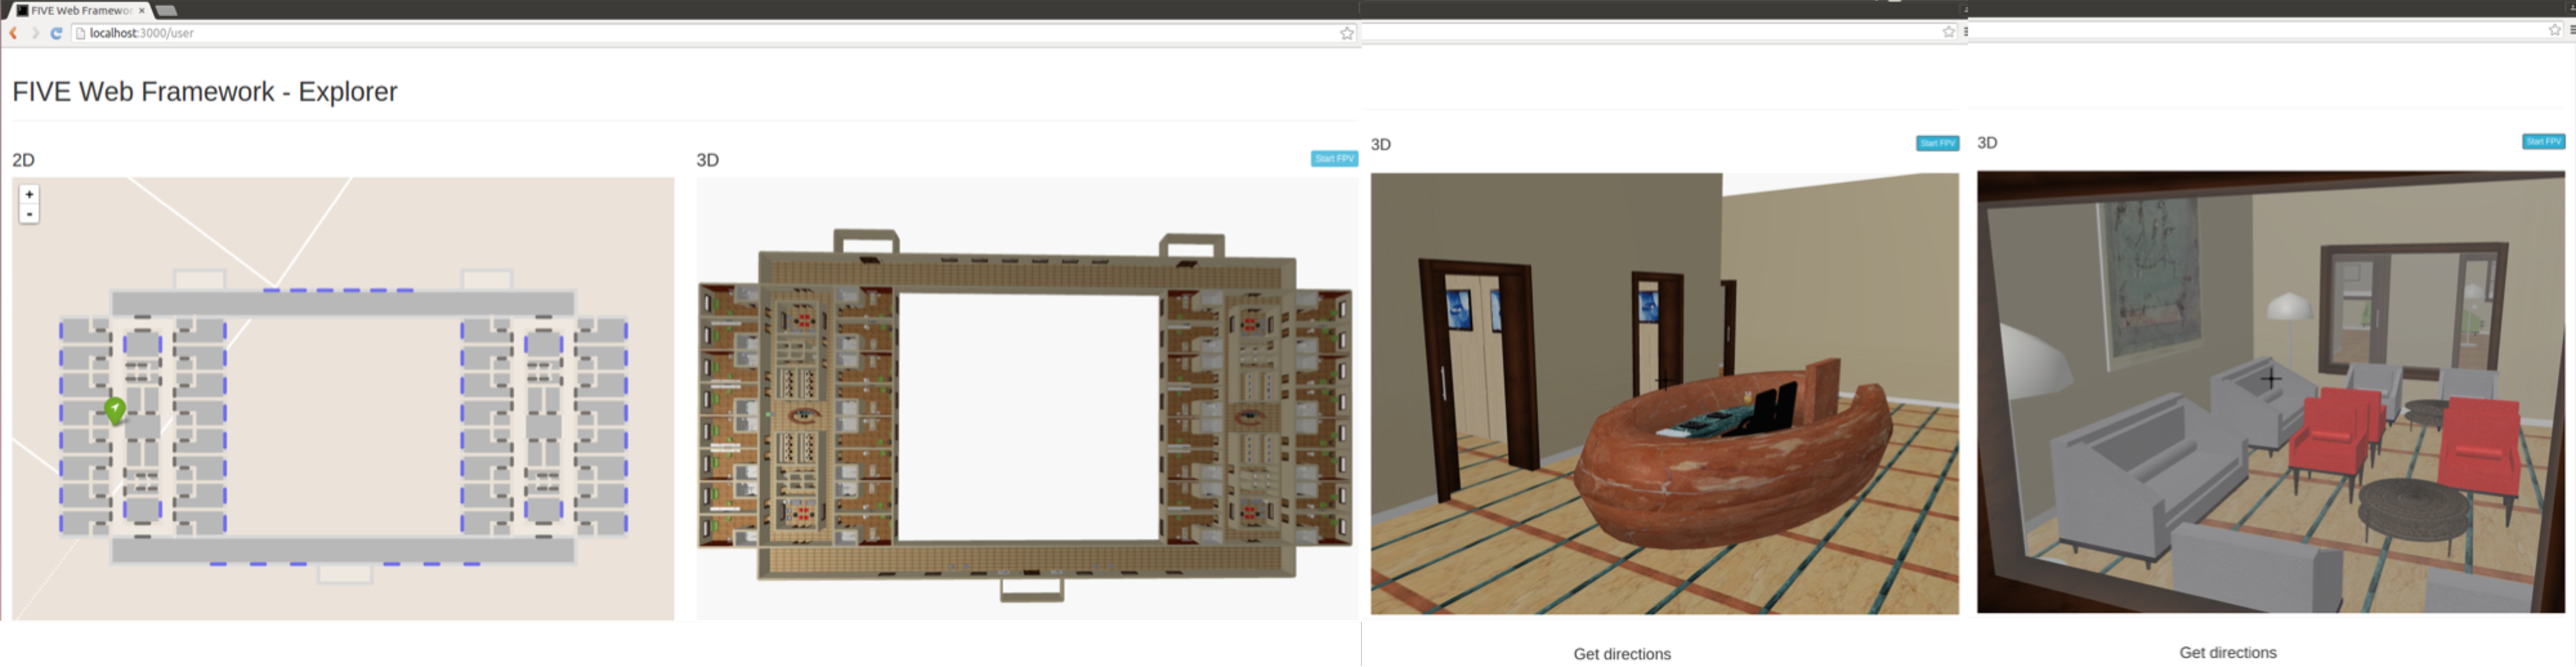
\includegraphics[width=\linewidth]{images/ward/ward} 
   
   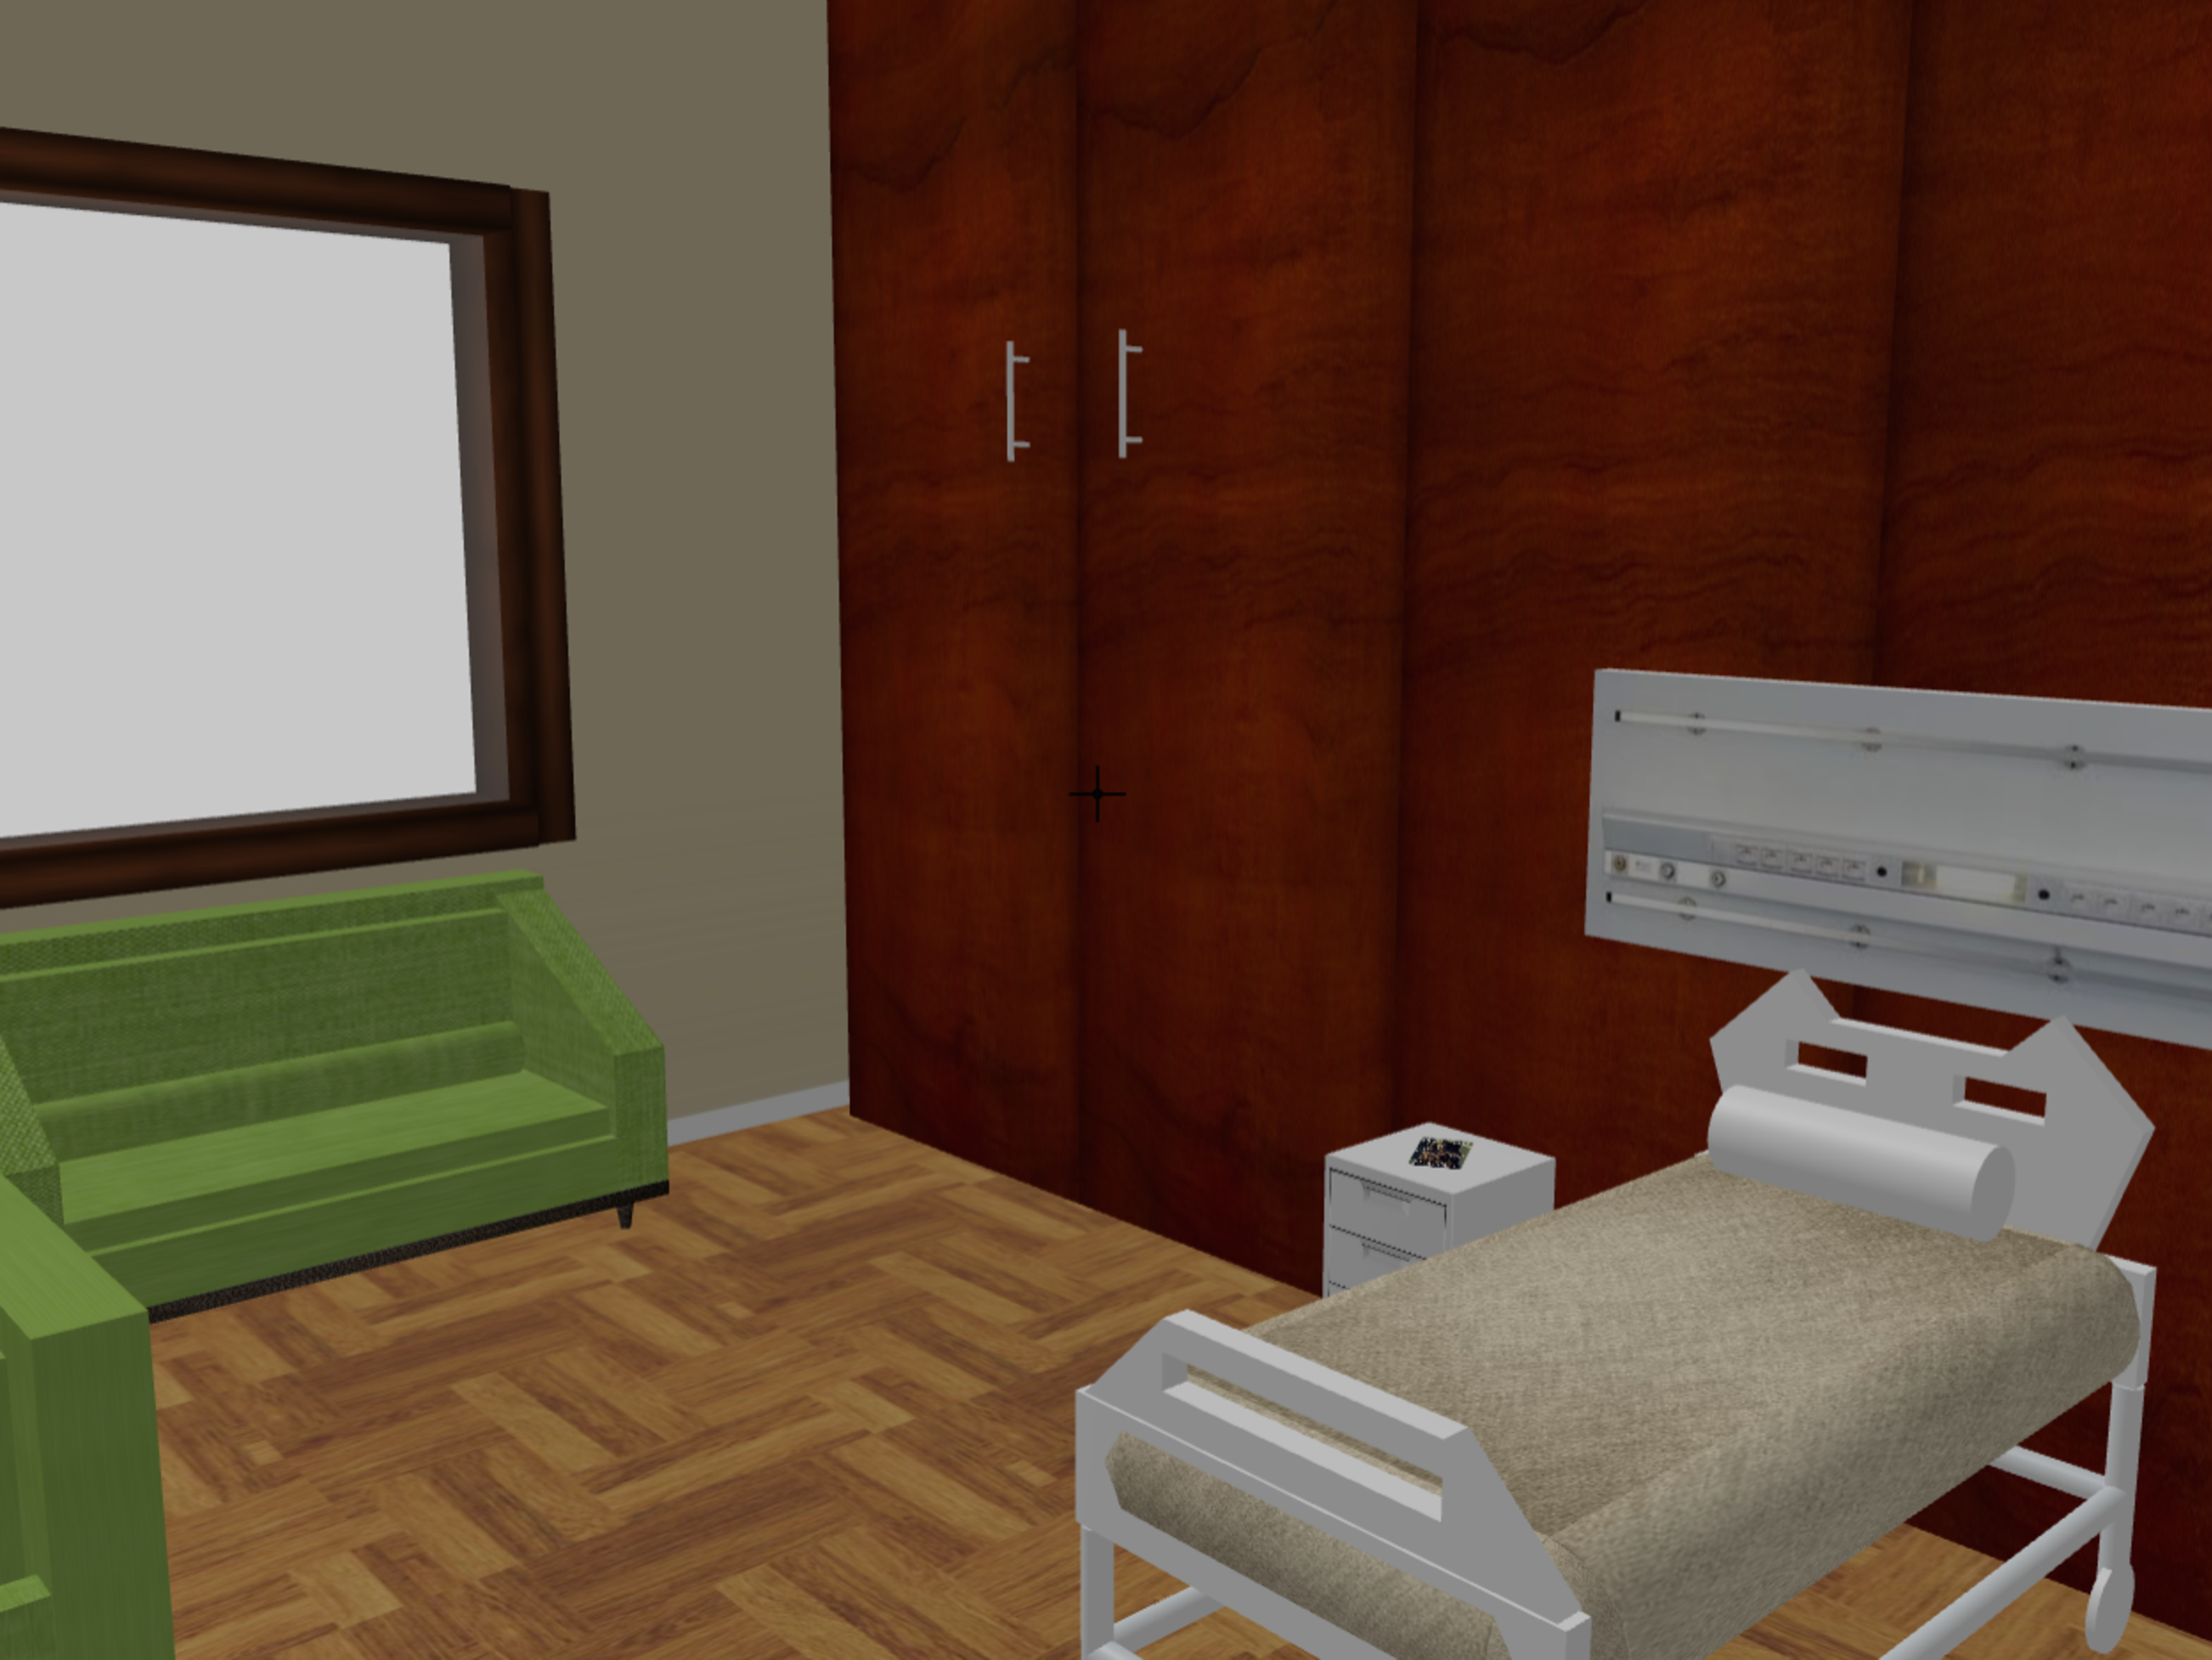
\includegraphics[width=0.327\linewidth]{images/ward/room} 
   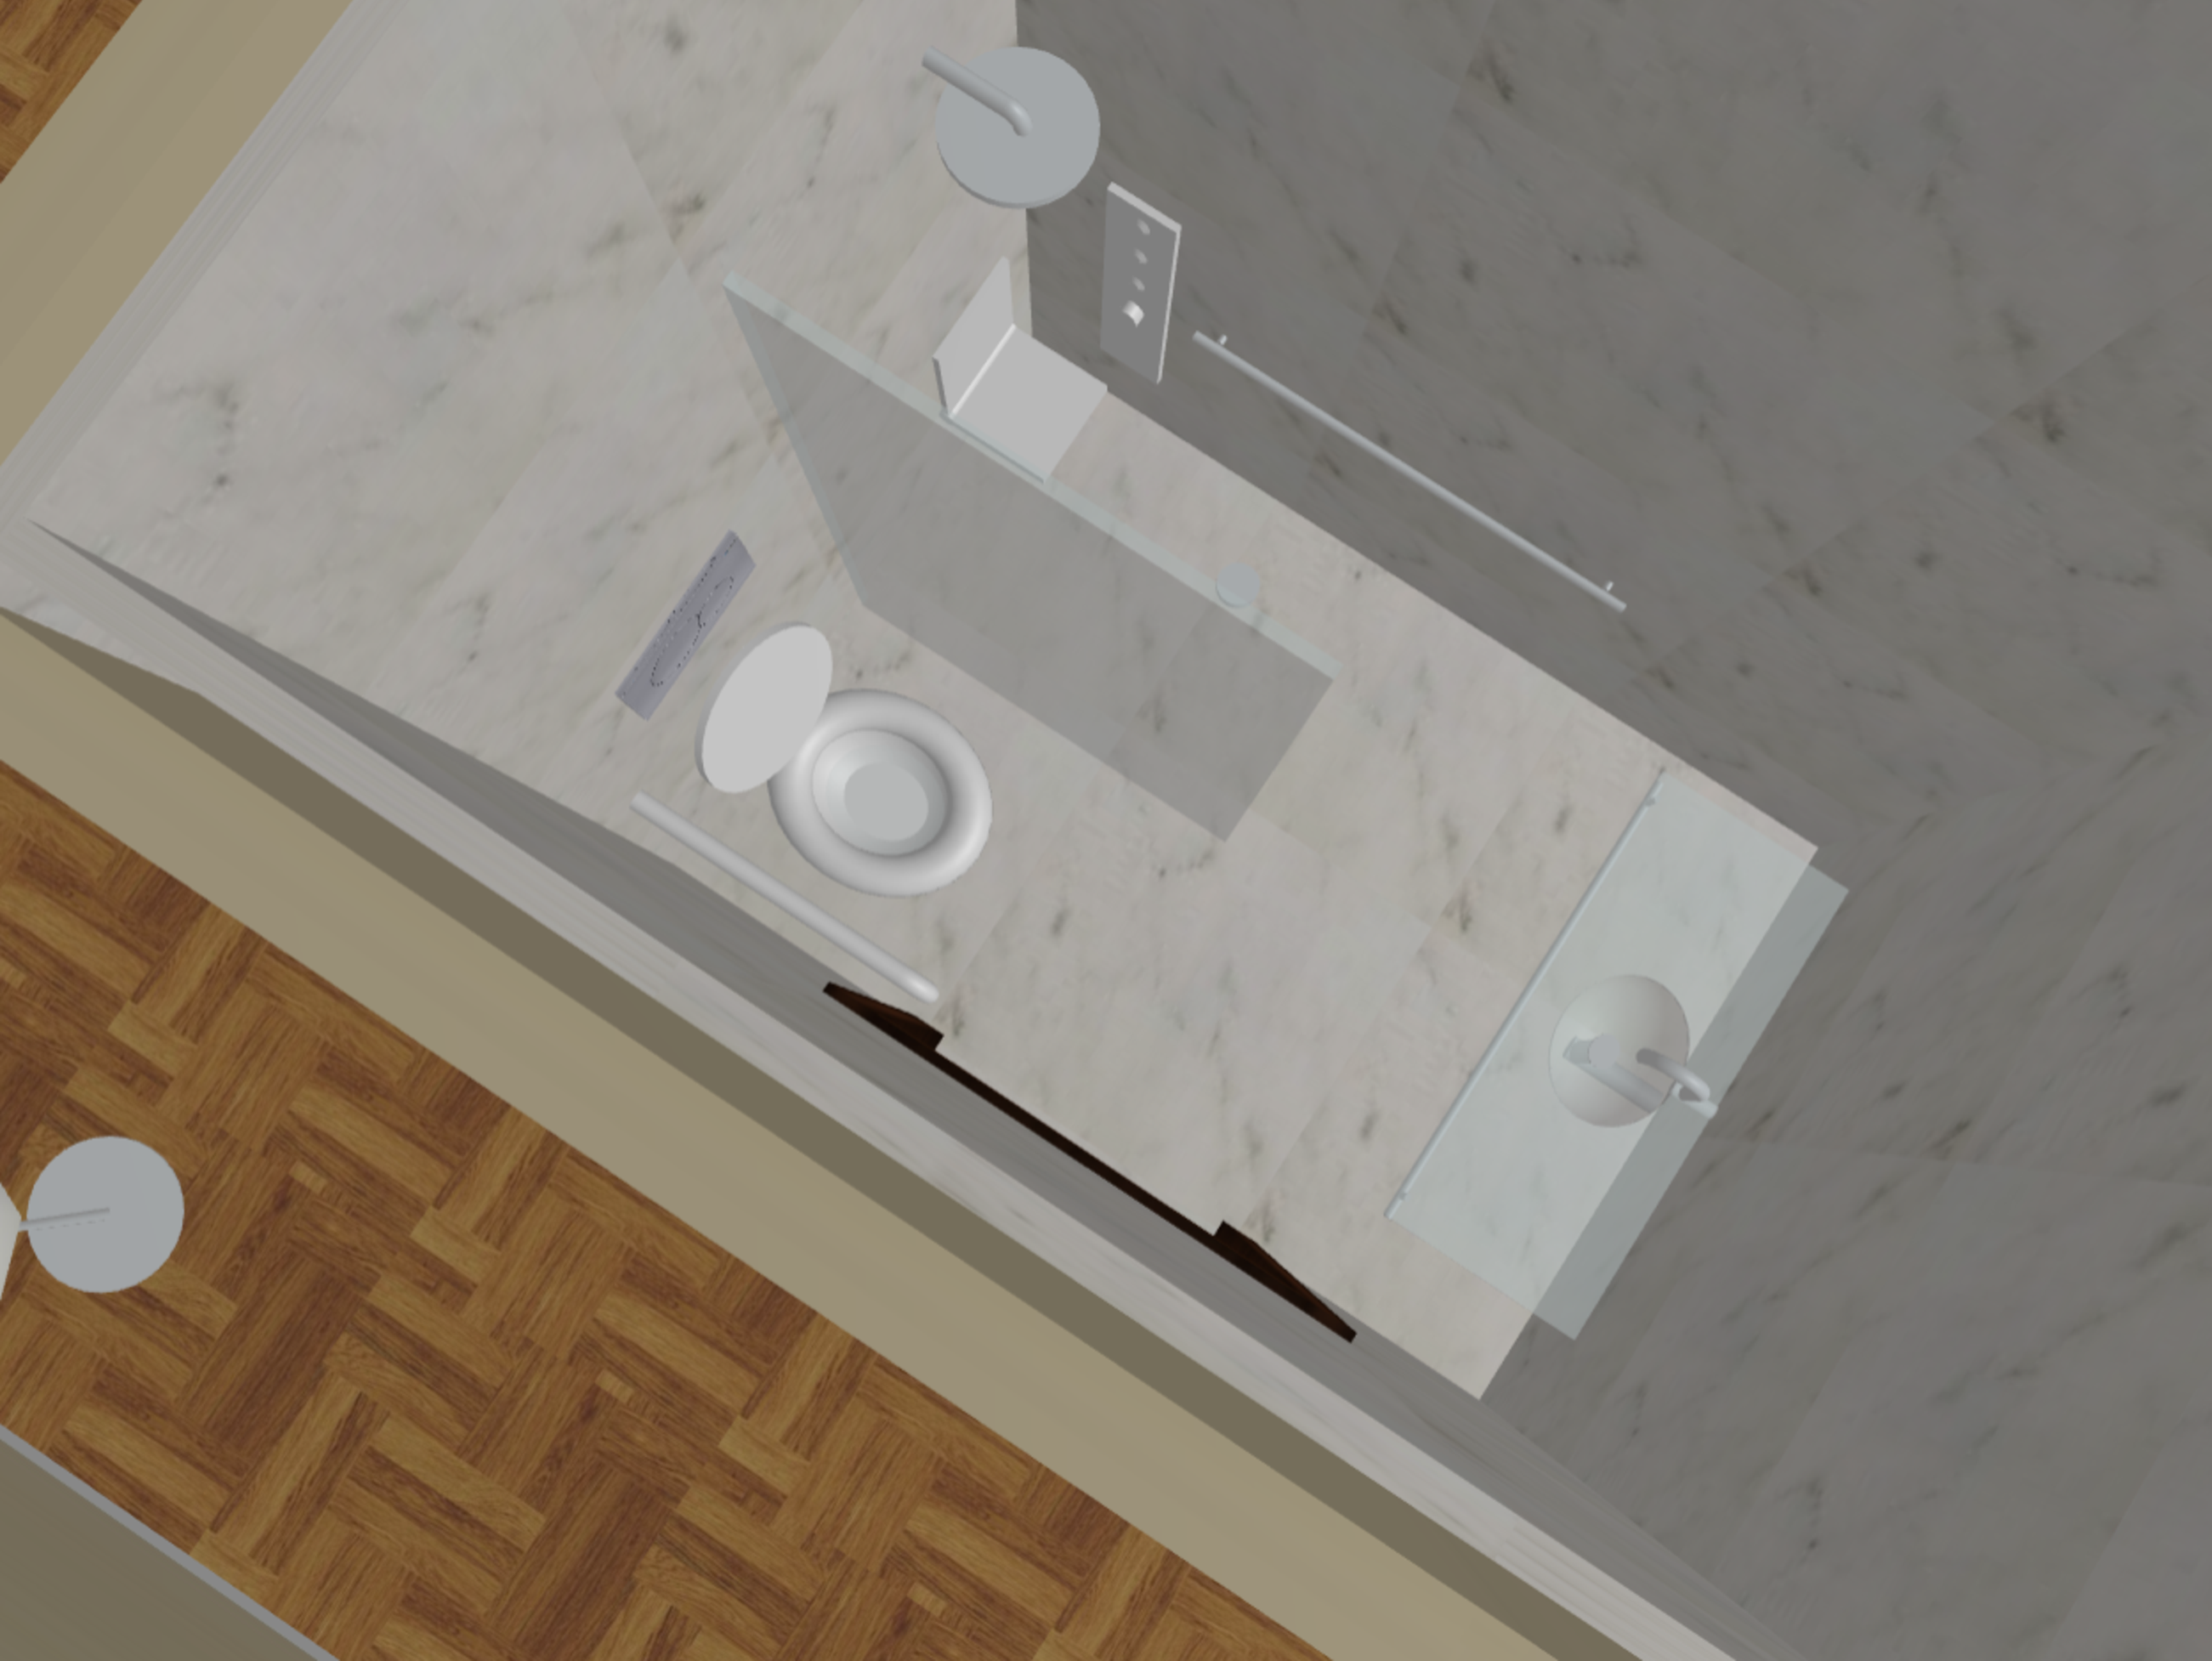
\includegraphics[width=0.327\linewidth]{images/ward/bath} 
   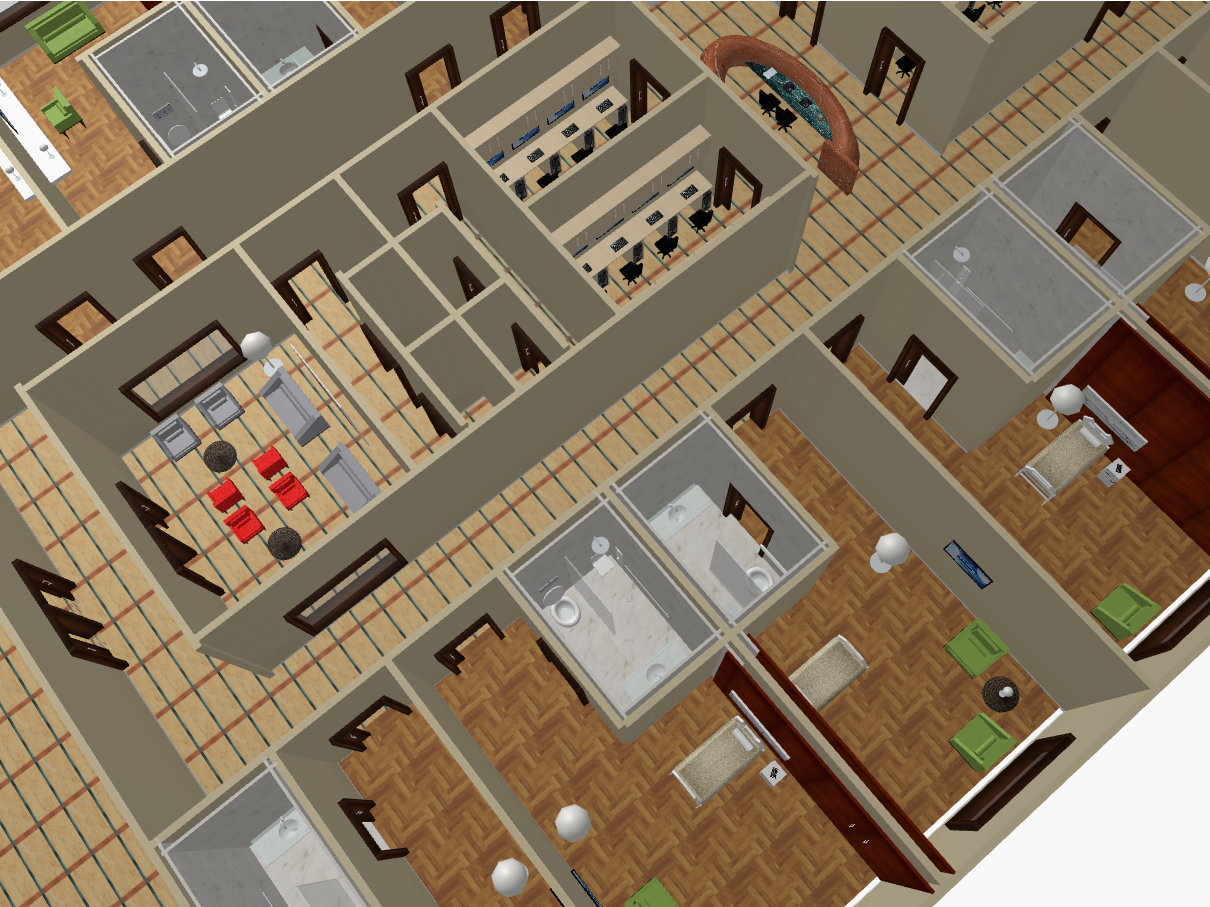
\includegraphics[width=0.327\linewidth]{images/ward/ward5} 
   \caption{Some images of two ward departments of an hospital design from an interactive session with the FIVE environment.}
   \label{fig:ward}
\end{figure*}



\begin{figure*}[ptb] %  figure placement: here, top, bottom, or page
   \centering
   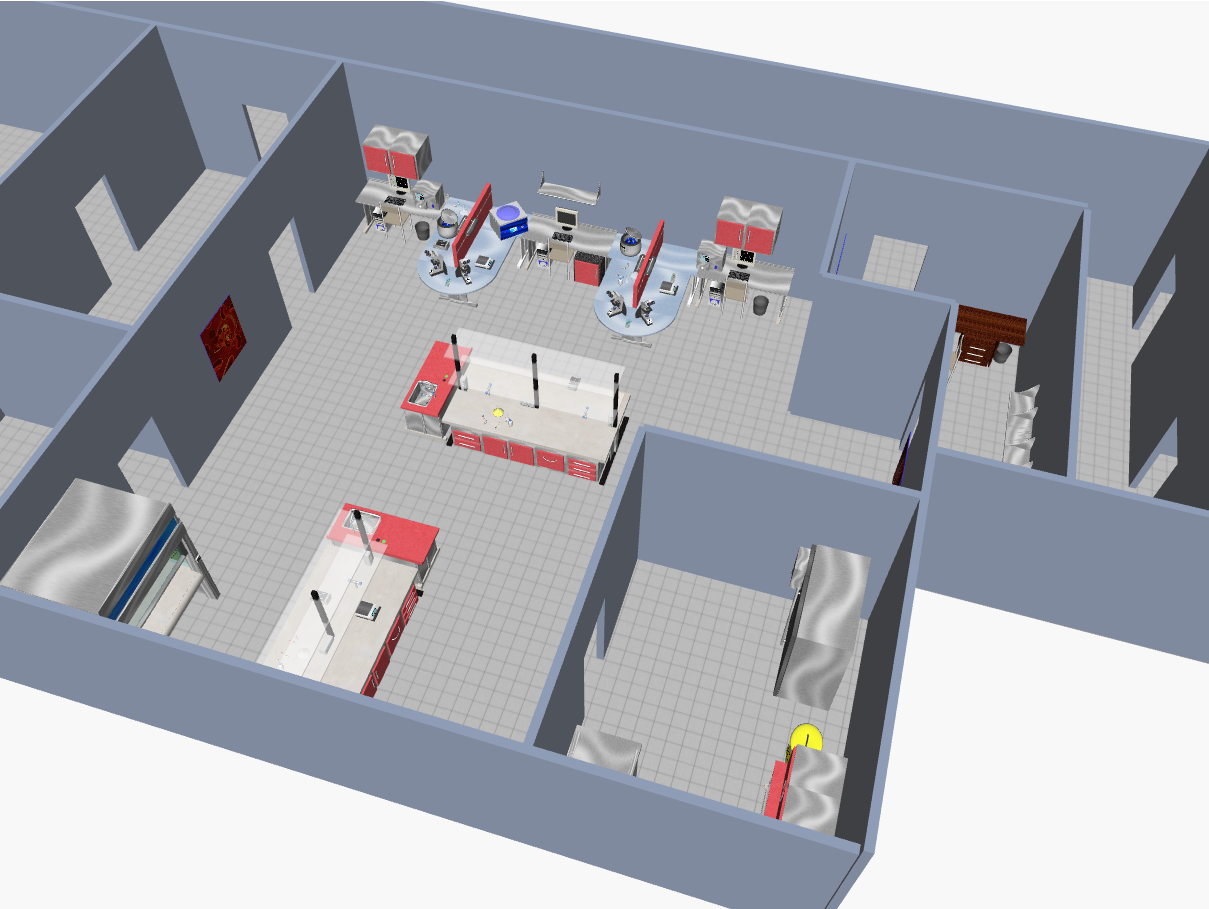
\includegraphics[width=0.327\linewidth]{images/lab/lab0} 
   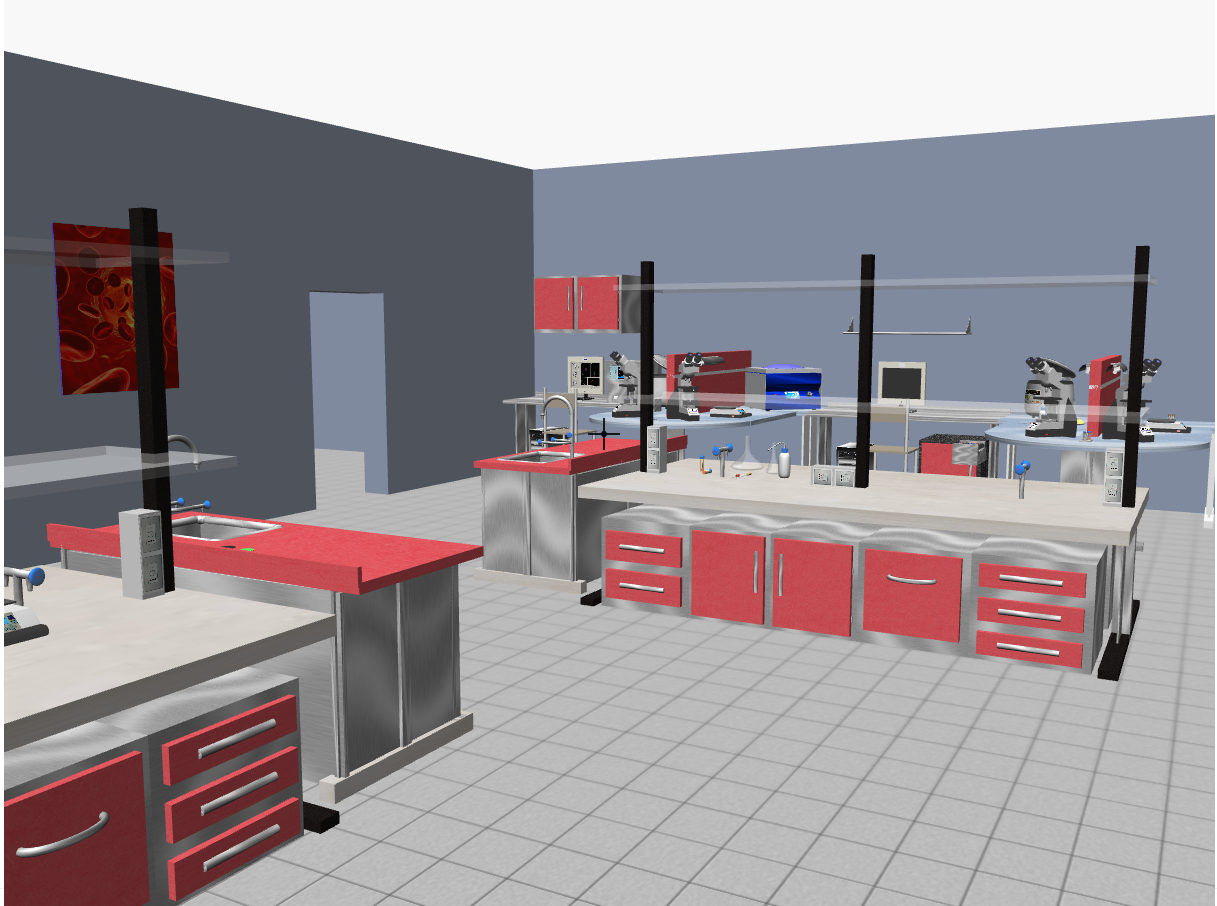
\includegraphics[width=0.327\linewidth]{images/lab/lab2} 
   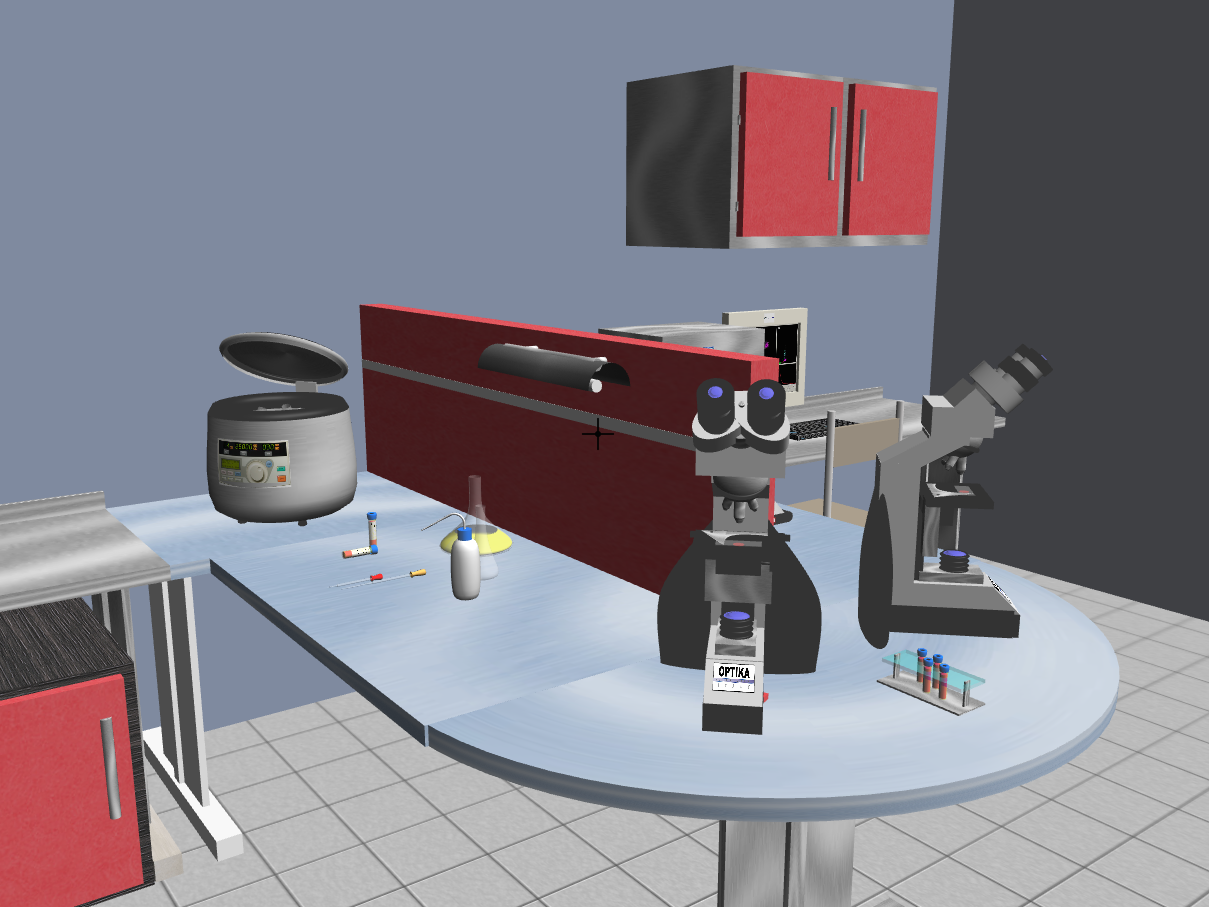
\includegraphics[width=0.327\linewidth]{images/lab/lab3} 

   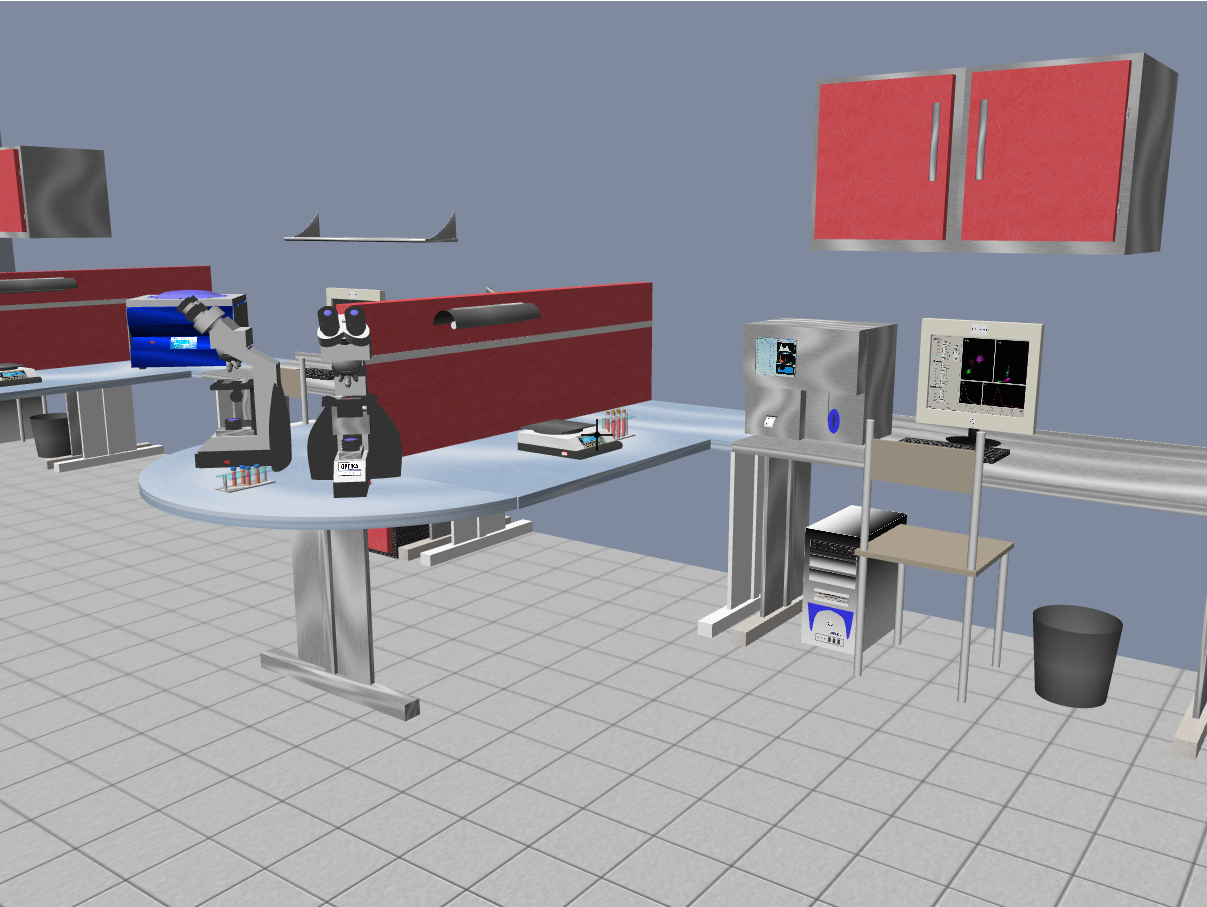
\includegraphics[width=0.327\linewidth]{images/lab/lab4} 
   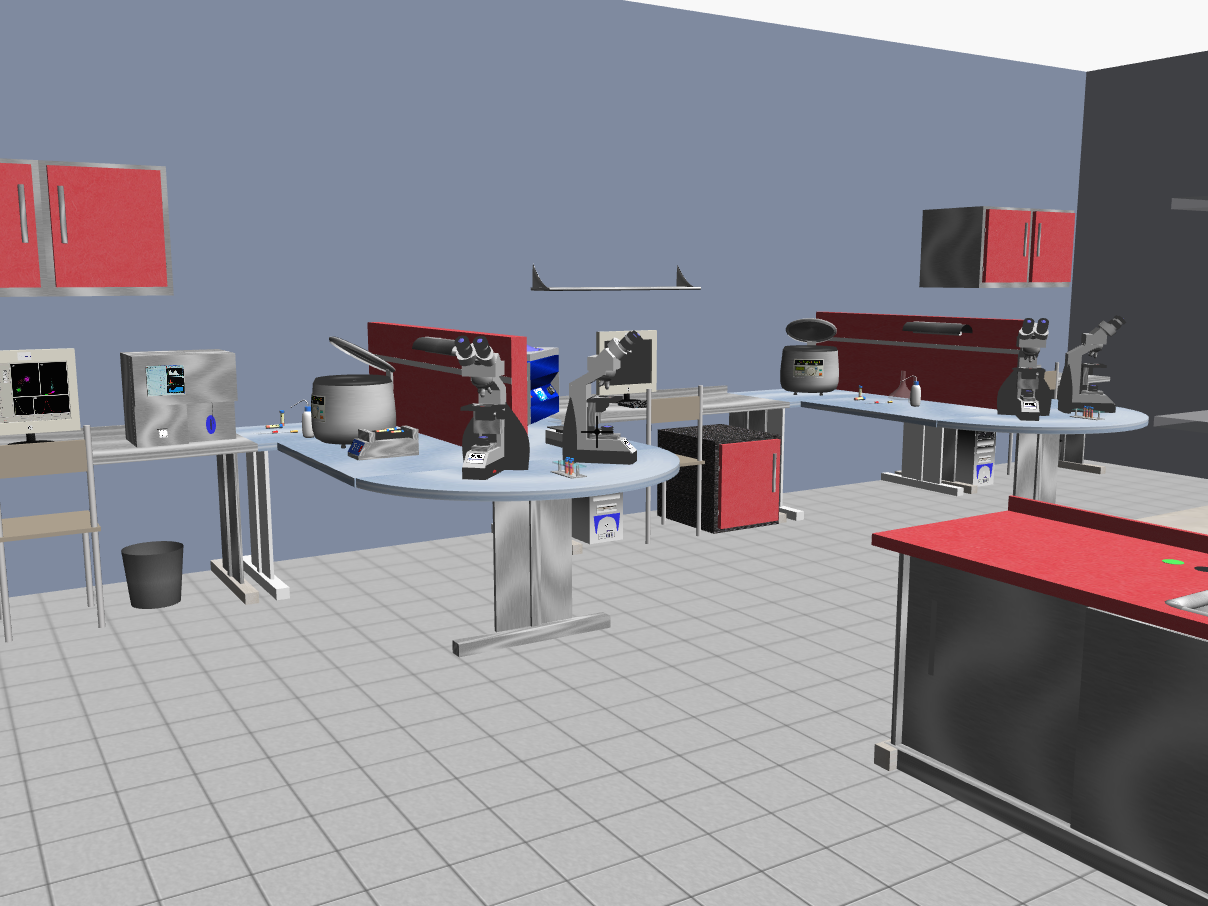
\includegraphics[width=0.327\linewidth]{images/lab/lab5} 
   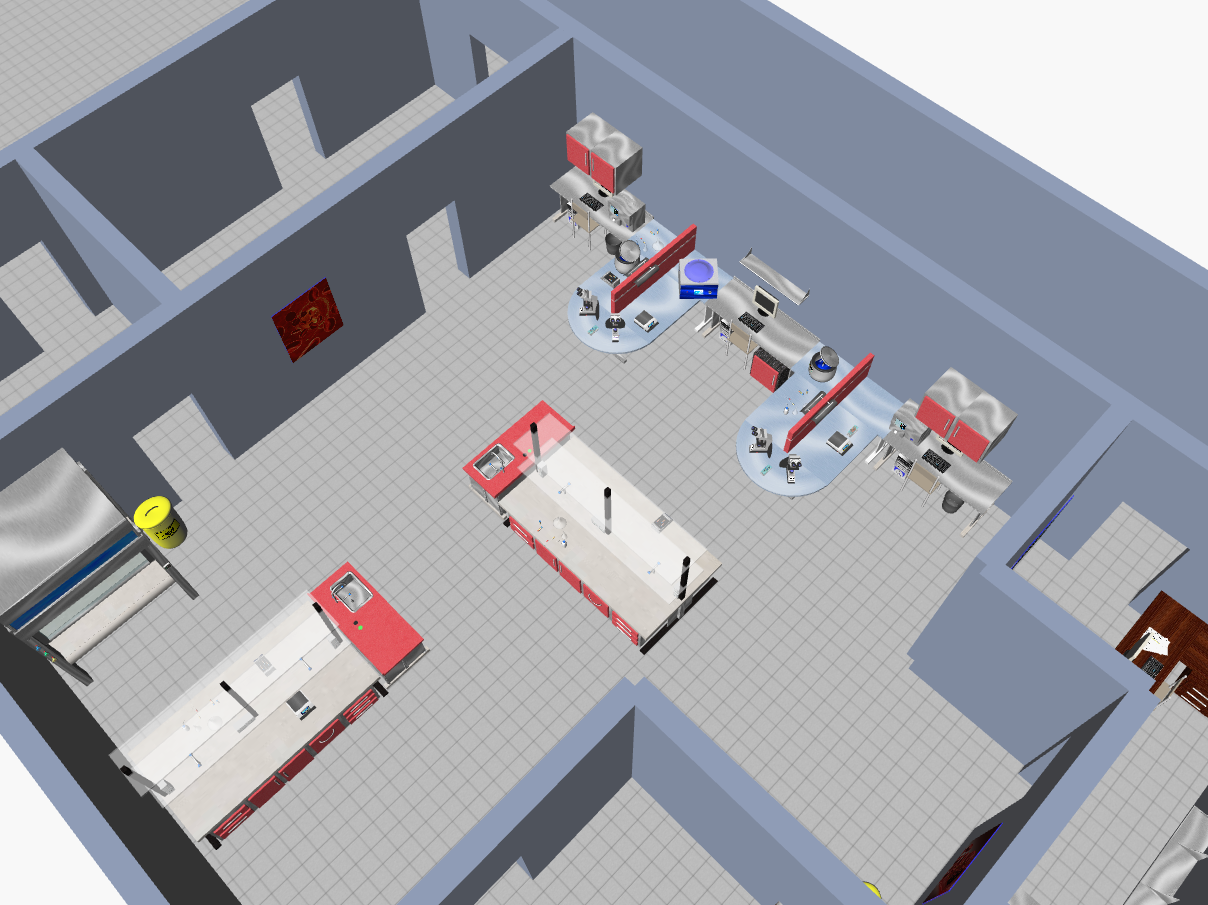
\includegraphics[width=0.327\linewidth]{images/lab/lab6} 
   \caption{Some images of the Laboratories department of an hospital design.}
   \label{fig:lab}
\end{figure*}


\begin{figure}[ptb] % figure placement: here, top, bottom, or page
 \centering
 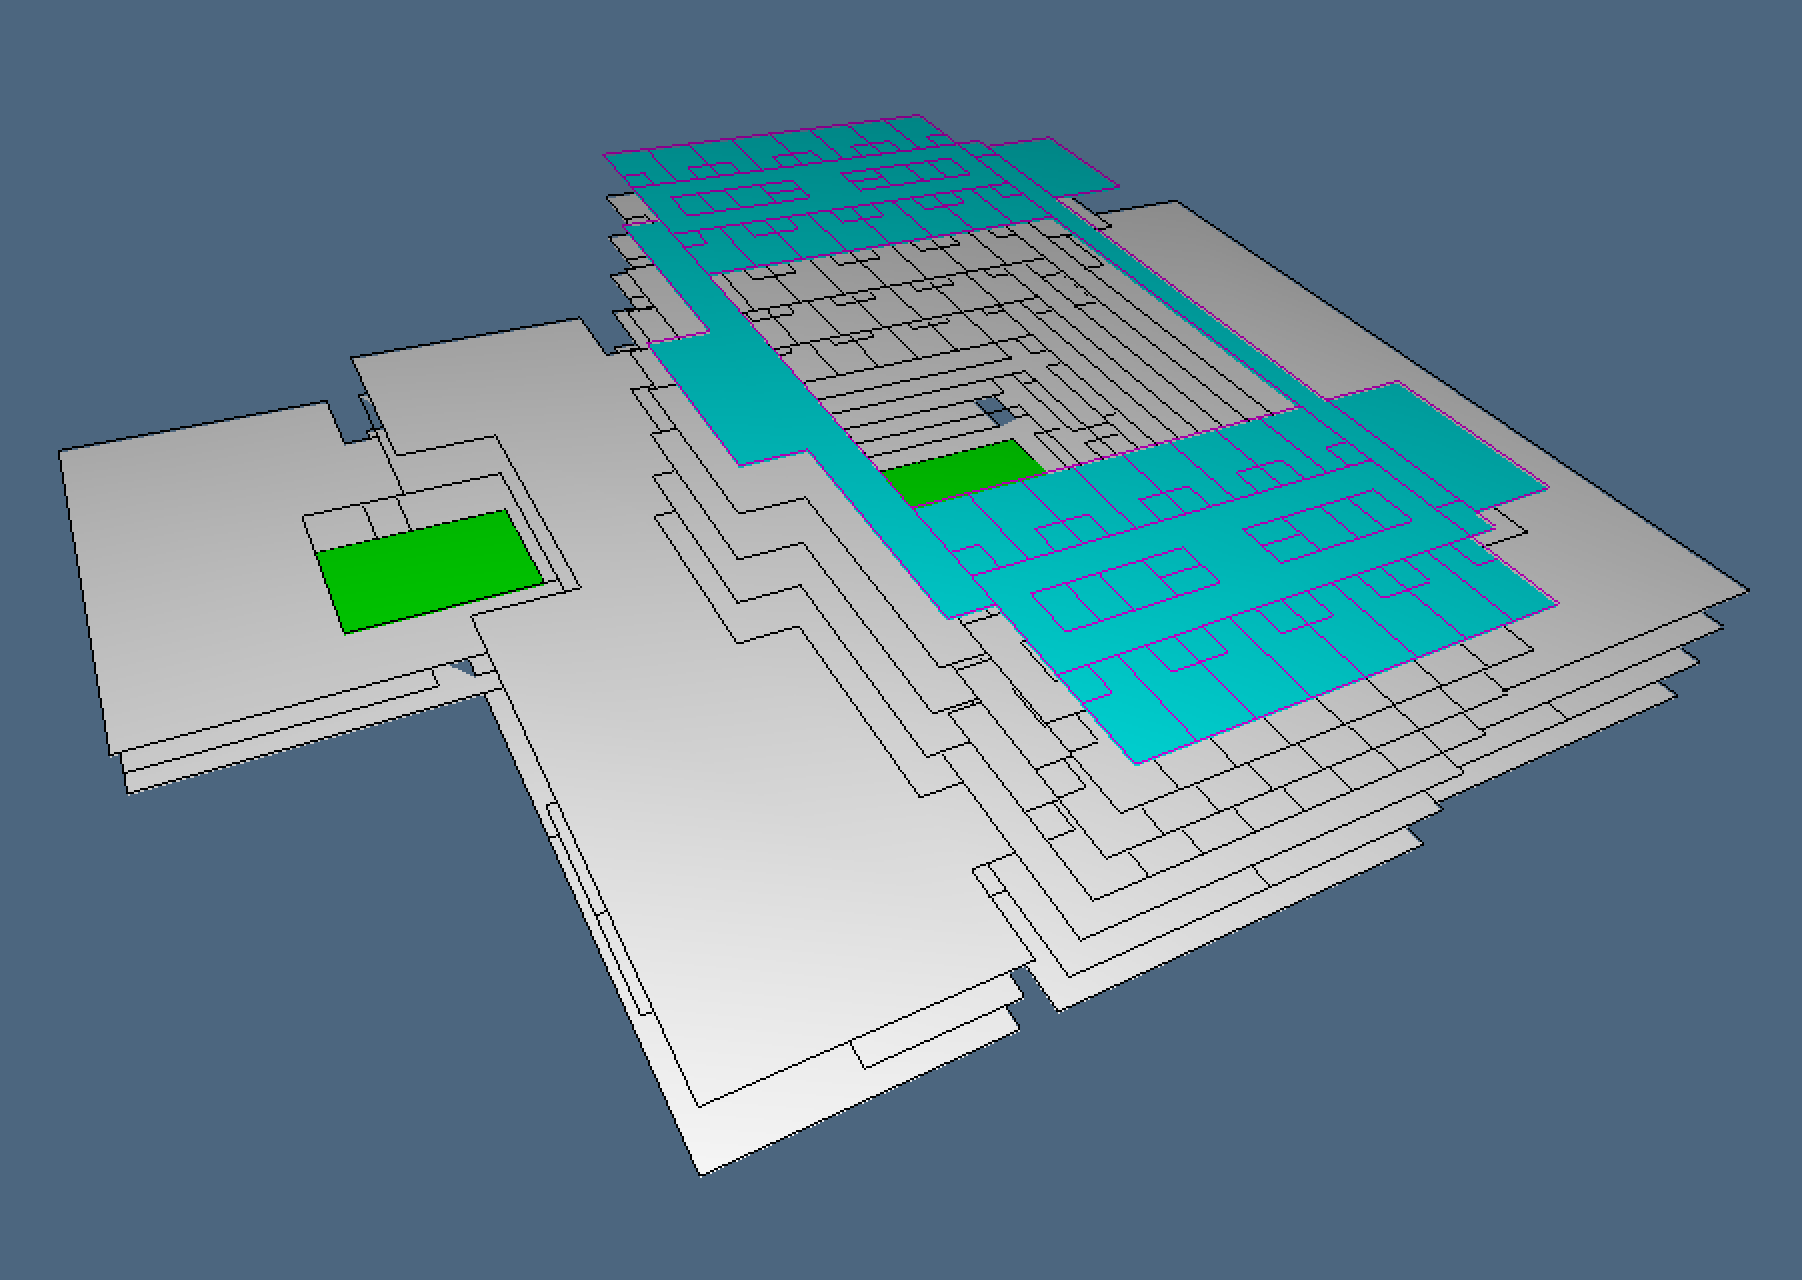
\includegraphics[width=\linewidth]{images/hospital2} 
 \caption{An image of the 2.5D model of a general hospital, defined as the LAR of a 2-complex embedded in 3-space. Notice that 2-cells may be non-convex. The cyan floor corresponds the pair of ward departments translated into the HIJSON format and displayed in Figures~\ref{fig:ward} and~\ref{fig:lab}.}
 \label{fig:hospital2}
\end{figure}

 The HIJSON  files are served on the web and transformed real-time client-side into the FIVE interactive interface (either 2D, or 3D or both) of the indoor mapping applications. The sequence of steps is outlined below:

1. \textit{Input of wire-frame drawings},
  starting from   raster \emph{images} of architectural floorplans of the building, interpreted into a simplified 2D vector representation (\texttt{.svg} files);

2. \textit{Generation of a 2D cellular complex}, via
  parsing of graphics elements from textual files, and automatic generation of a 2D cellular complex for topological computations and long-term storage of the model (\texttt{.lar} files) using a very simple and general geometric format (LAR) based on algebraic topology and linear algebra with compressed sparse matrices (see Appendix~\ref{sec:lar});

3. \textit{Structured 2.5D description}, produced by
  hierarchical modeling of cellular models, through automatic transformation of grouping elements of \texttt{.svg} files into a 2D description providing \emph{semantics} to spaces and  to the various elements of the building fabric (vertical or horizontal external envelope, internal partitions, horizontal floors, vertical communications), by using an object-oriented hierarchical description as a  \texttt{Struct} network;

4. \textit{Exporting to HIJSON file}.
The  structured and semantically annotated 2.5D building model is finally  exported as a rich textual description into \texttt{HIJSON} files, i.e.~in JSON format, though and intermediate \texttt{.yml} translation;

5. \textit{Client-based processing}
  The \texttt{.json} files are finally transformed client-side into 
  2D and/or 3D virtual environments, allowing the real-time spatial placement and
  user-tracing within the virtual environment of the individuals moving
  inside the real building (see Figures~\ref{fig:ward} and~\ref{fig:lab}).



% \section{Case study}\label{case-study}

\begin{figure*}[ptb] %  figure placement: here, top, bottom, or page
   \centering
   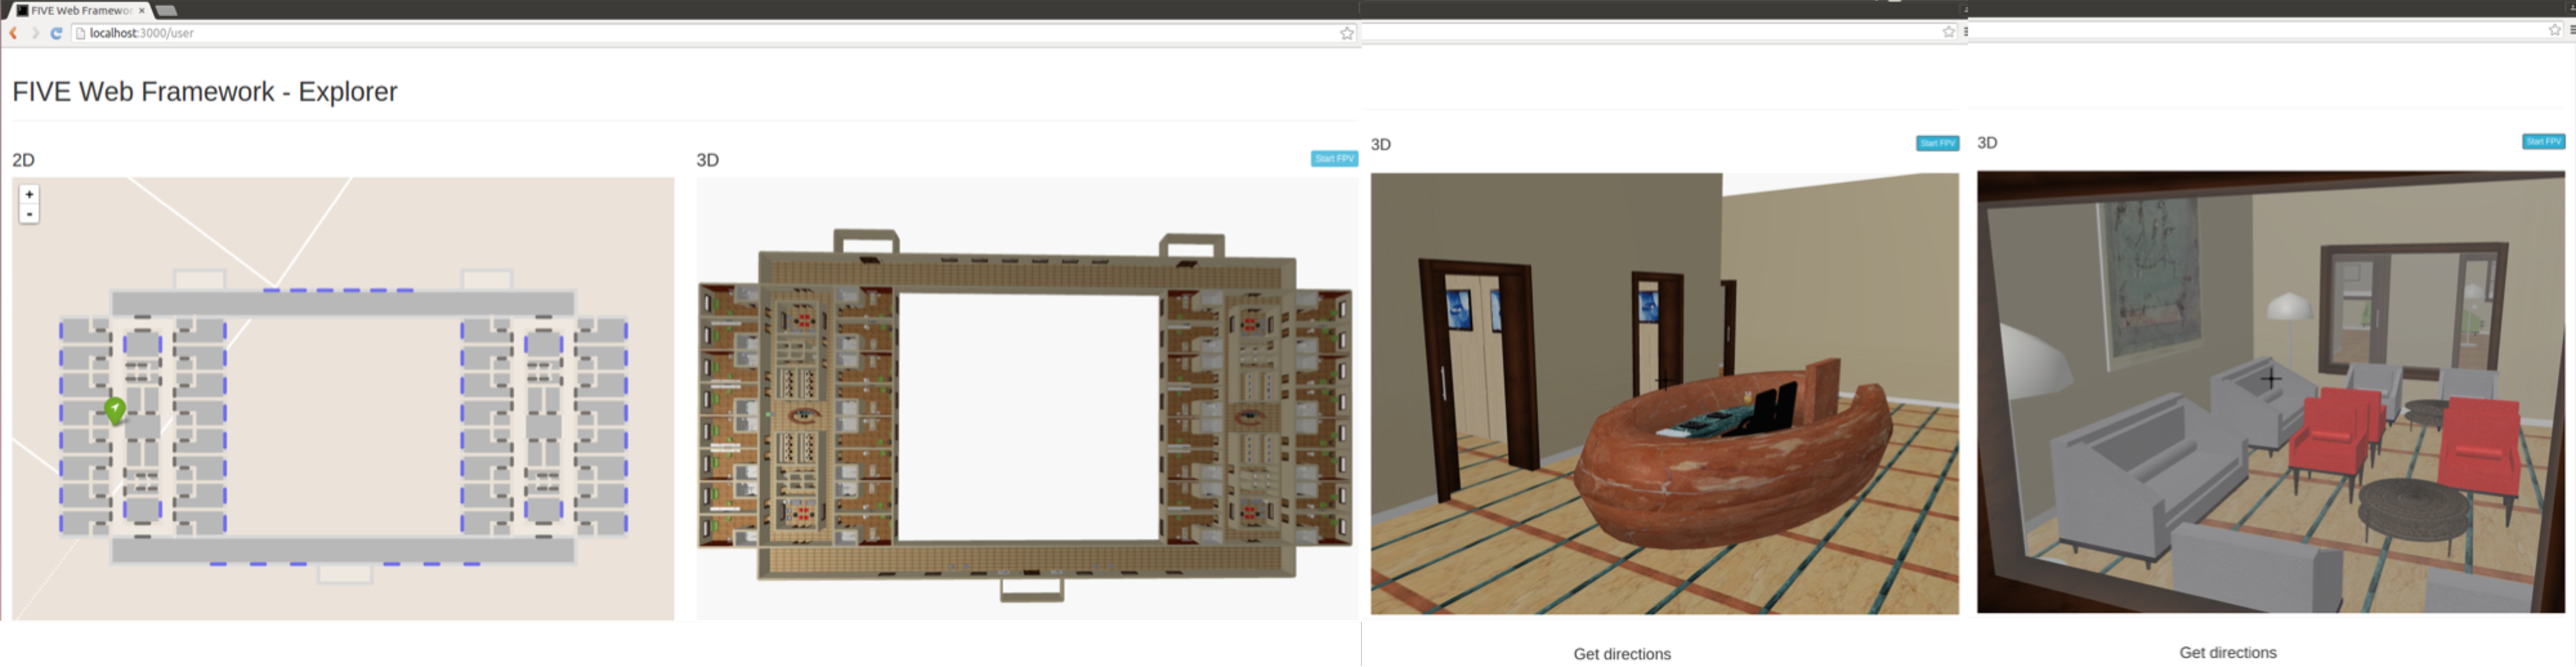
\includegraphics[width=\linewidth]{images/ward/ward} 
   
   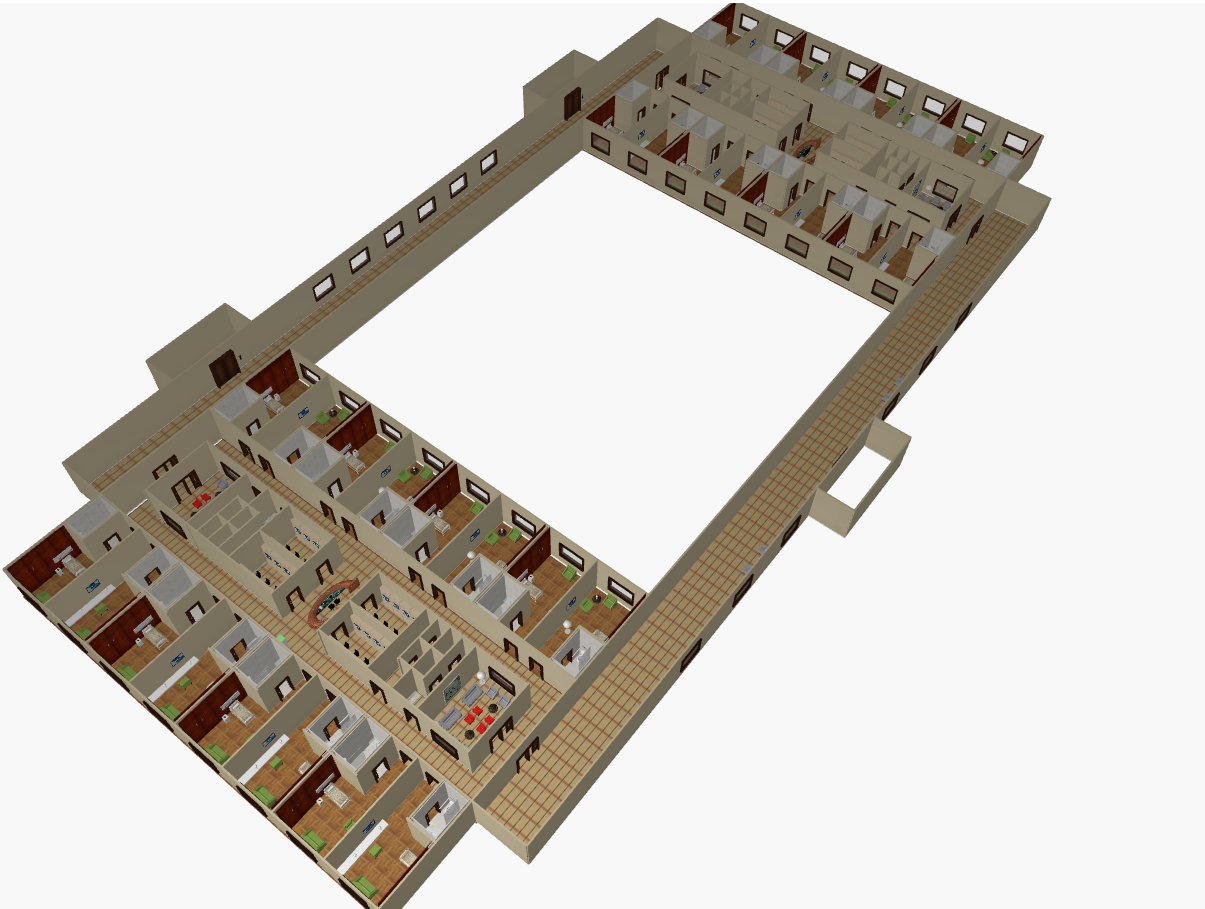
\includegraphics[width=0.327\linewidth]{images/ward/ward1} 
   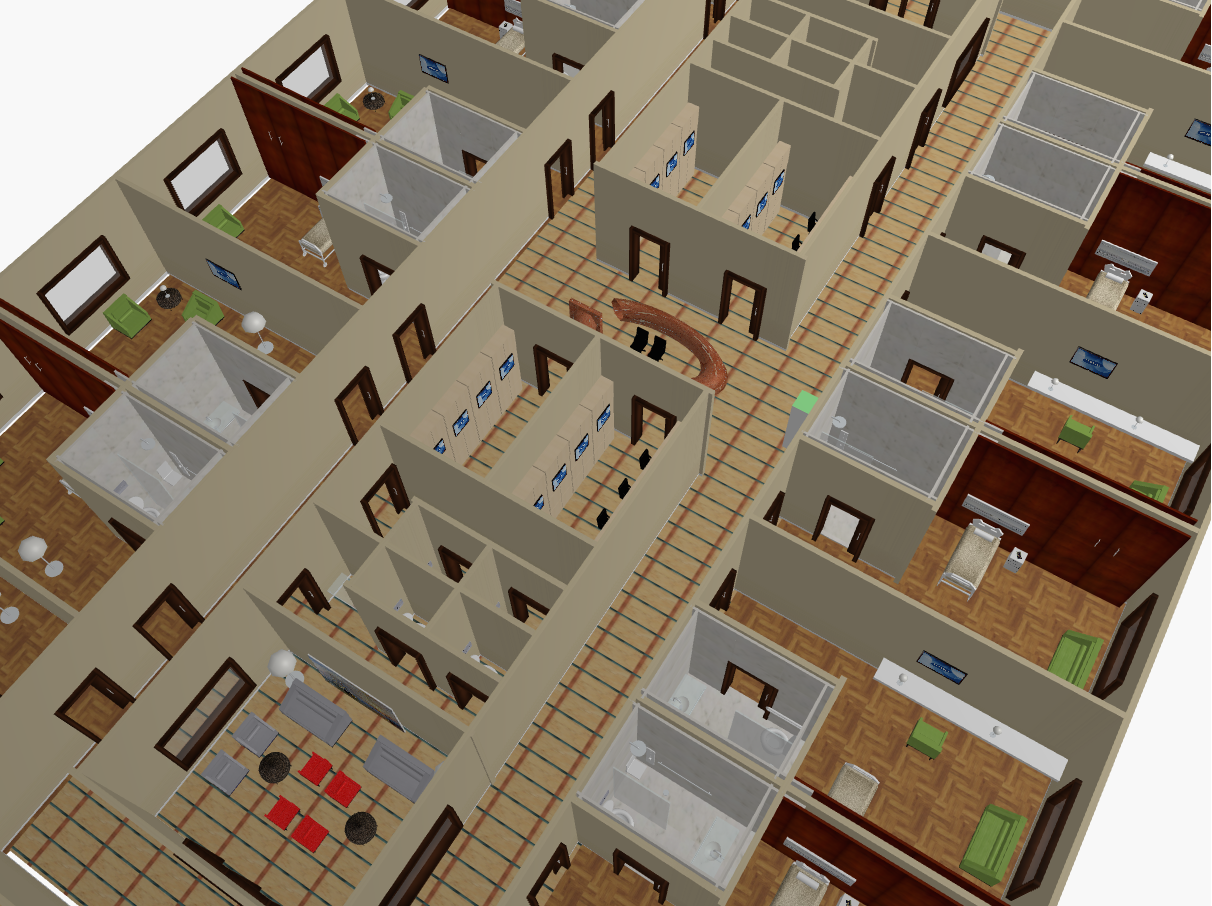
\includegraphics[width=0.327\linewidth]{images/ward/ward4} 
   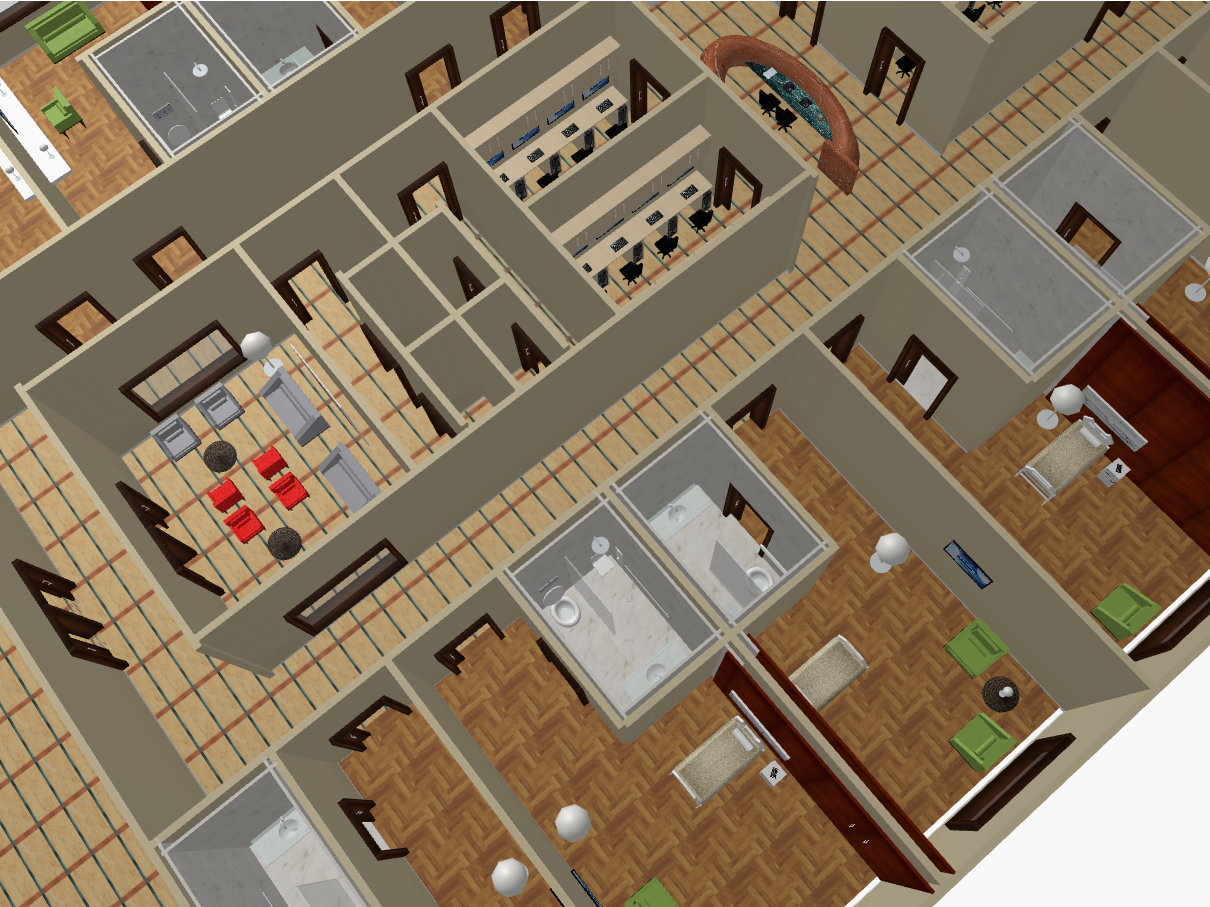
\includegraphics[width=0.327\linewidth]{images/ward/ward5} 
   \caption{example caption}
   \label{fig:example}
\end{figure*}



\begin{figure*}[ptb] %  figure placement: here, top, bottom, or page
   \centering
   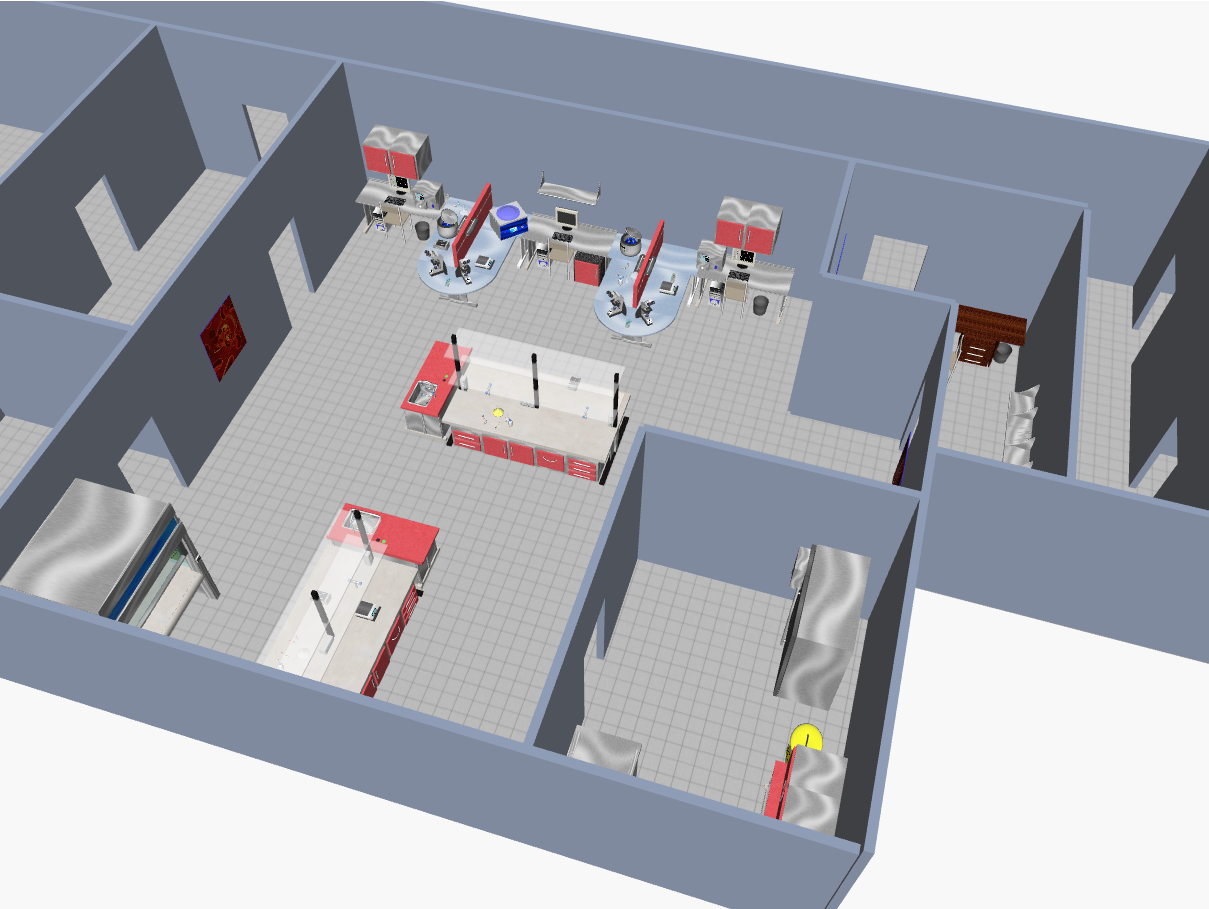
\includegraphics[width=0.327\linewidth]{images/lab/lab0} 
   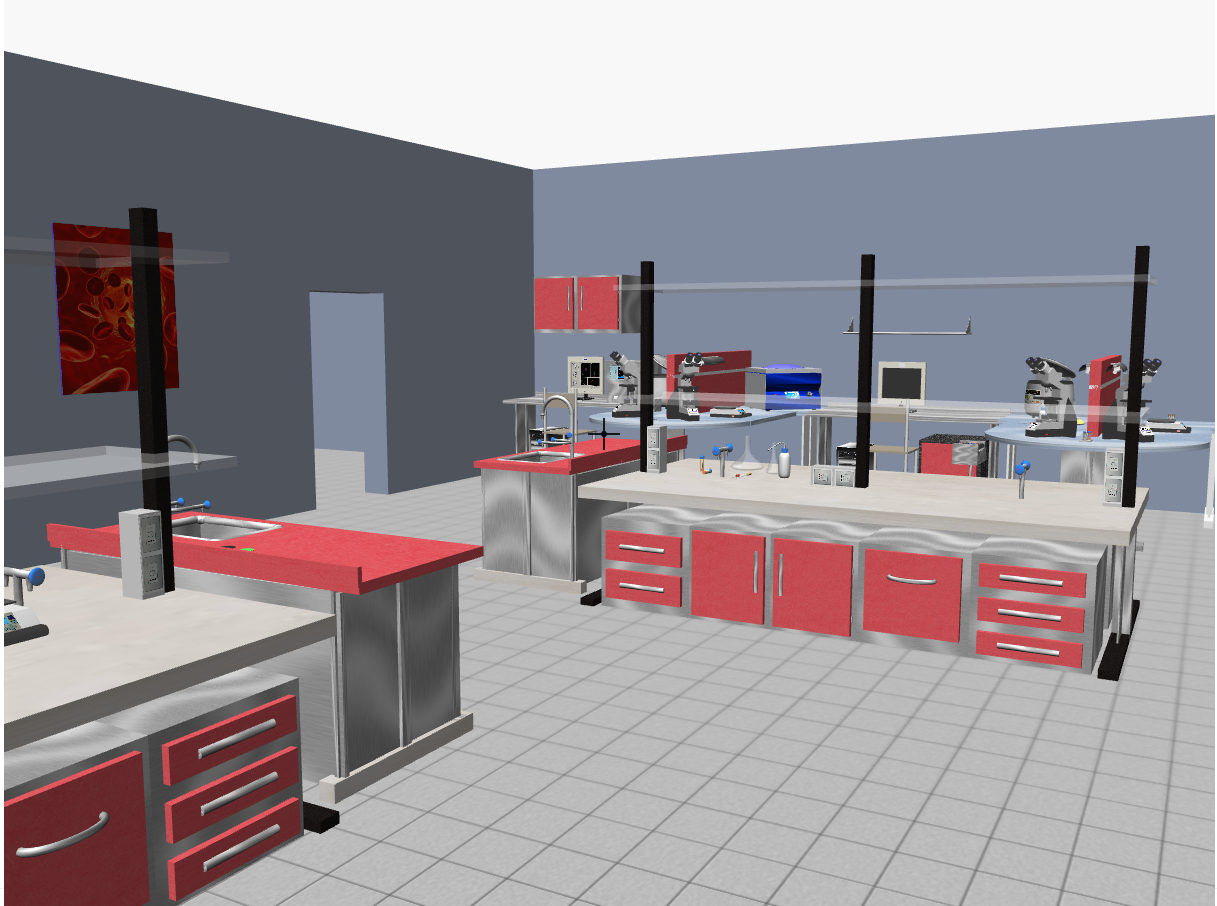
\includegraphics[width=0.327\linewidth]{images/lab/lab2} 
   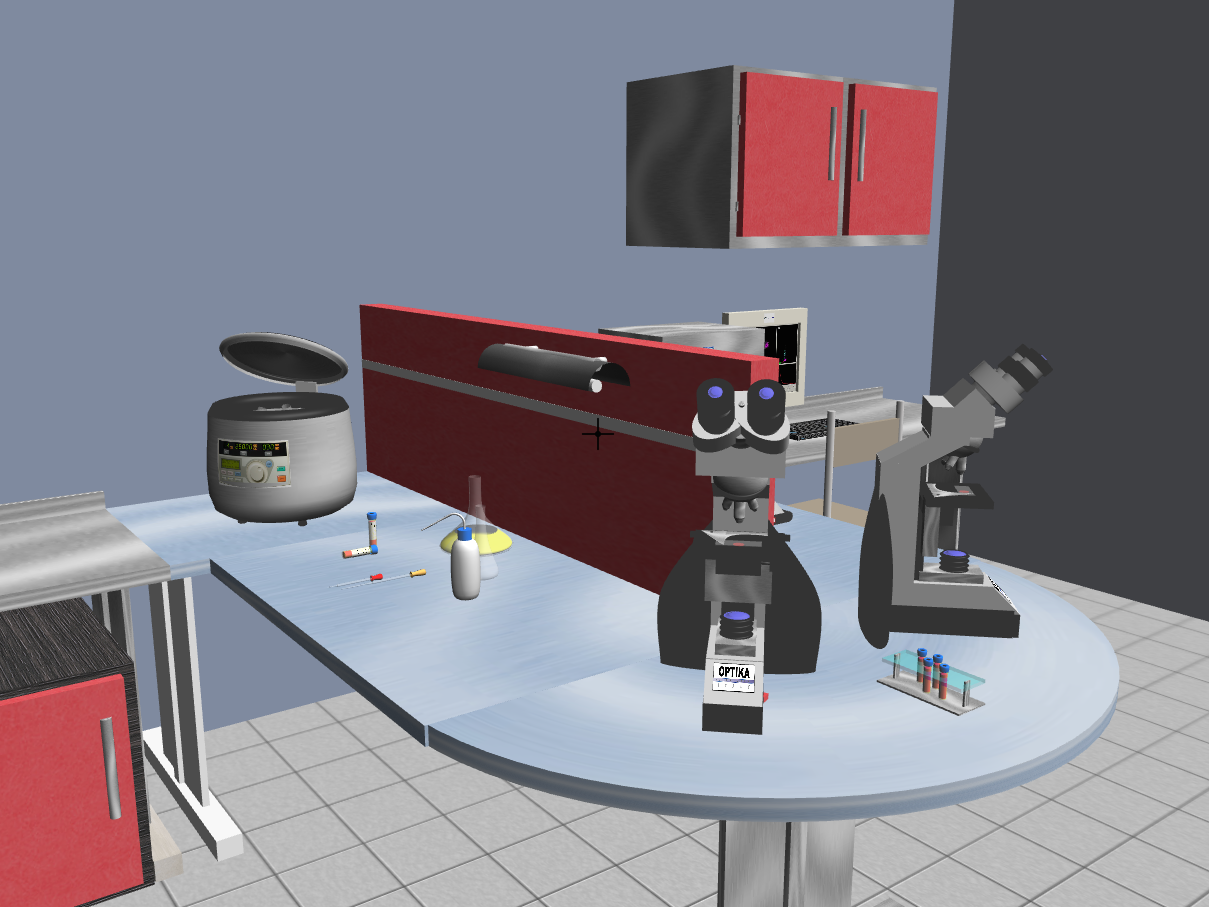
\includegraphics[width=0.327\linewidth]{images/lab/lab3} 

   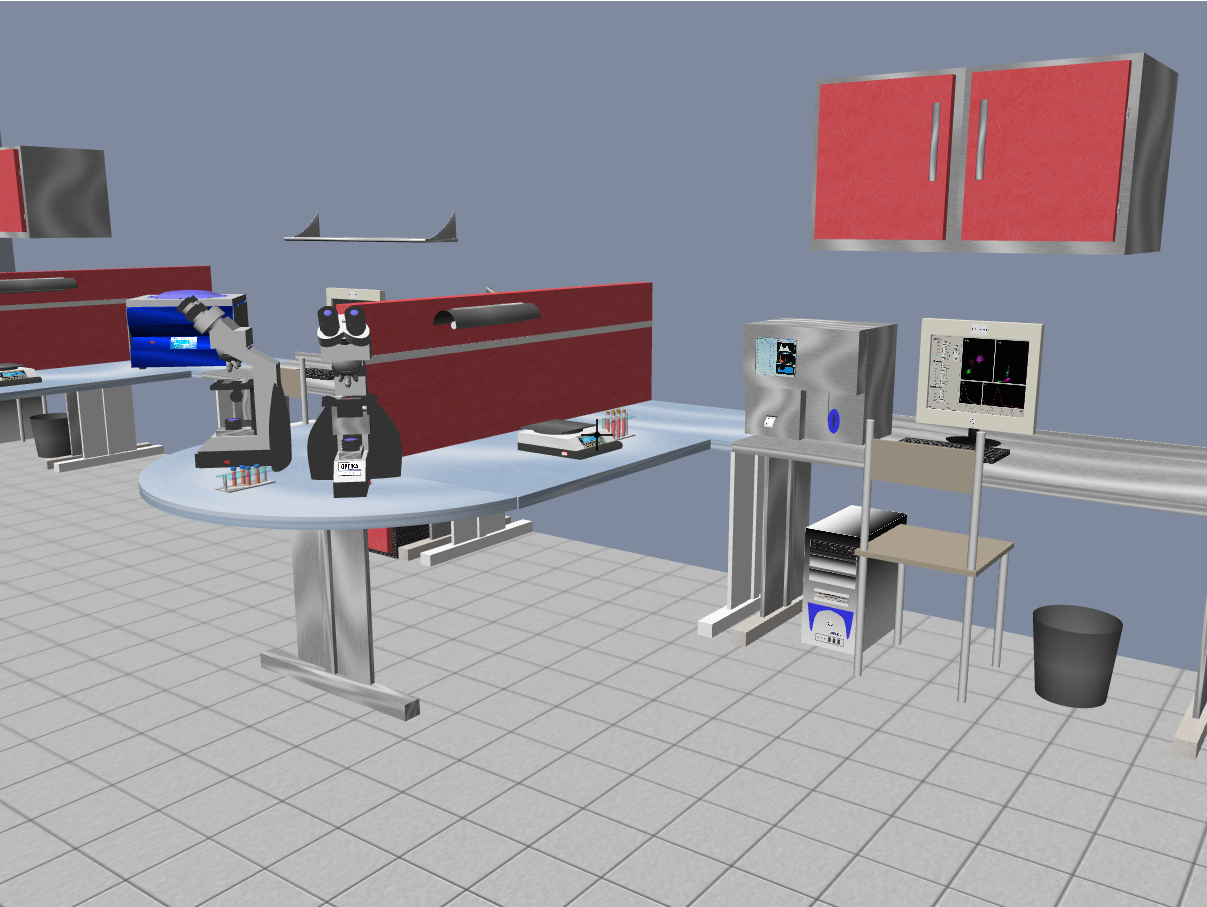
\includegraphics[width=0.327\linewidth]{images/lab/lab4} 
   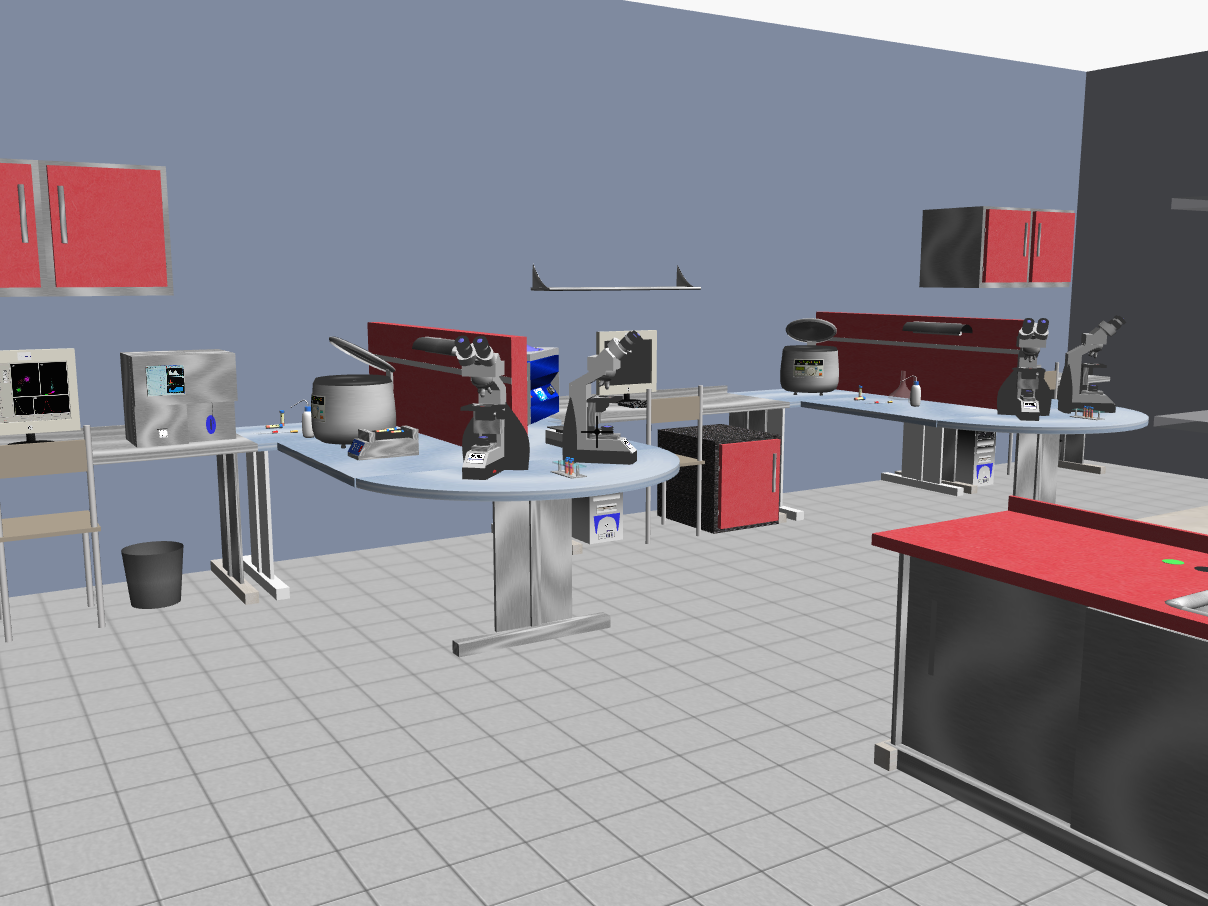
\includegraphics[width=0.327\linewidth]{images/lab/lab5} 
   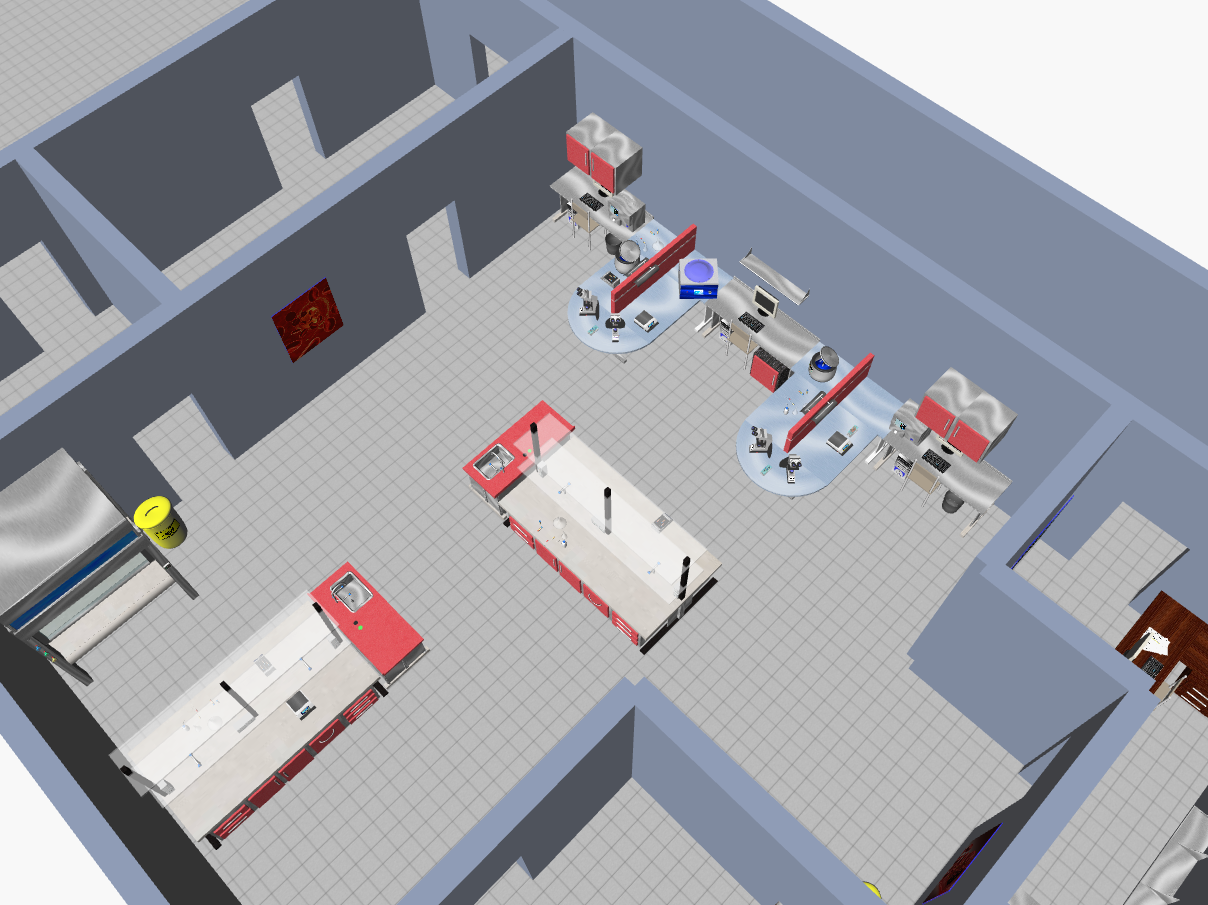
\includegraphics[width=0.327\linewidth]{images/lab/lab6} 
   \caption{example caption}
   \label{fig:example}
\end{figure*}

As case study of the discussed approach, we have taken into account the need of Sogei S.p.A. to support its maintenance service  workflow, since its data center, one of biggest data centers in Europe, is subject to very strict access control policies. 

The overall state of the data center can be monitored through the \emph{Supervisor} client. In this case the considered smart objects belong to a range of different devices, going from webcams, that provide on request the captured video streams, by way of alarm and antifire systems, till to individual servers, that can be monitored along several dimensions, including operating temperature, workload, etc. 

The most common maintenance scenario consists of an intervention by a technician that have to move across the environment, and locate within a huge data center the machine on which to operate, a not trivial task due to the presence of thousands of similar-looking machine racks. Thus the operator will be equipped with an \emph{Explorer} client, which will drive him to the target machine on which operate, while continuously notifying to a security \emph{Supervisor} his position, obtained by interacting with the indoor positioning system.
The maintenance workflow supervisor, using the \emph{Supervisor} client, is able to monitor the operator position within the data center, verifying that he does not deviate on unauthorized paths, triggering some console alarm if this happens.

The purpose is to support  the process of those in charge of carrying out the ``ticket-maintenance'' activities, as quickly  as possible and without error. The ``maintenance man'' will be guided to the right sub-system among thousands of racks. The real-time awareness of the relative positions between the ``maintenance man'' and the rack --- containing the sub-system --- will help to reduce intervention times and to increase safety. By  knowing when the maintenance process starts, the system  can automatically move, in real time, services, which are hosted on virtual machines, to other systems, thus maintaining the continuity of services and, at the same time,  reducing  the global risk factor. When the ``ticket-maint\-enan\-ce'' is over, and the technician goes away, it is possible to immediately  restore  the pre-existing conditions of services after a complete test has been performed.




%----------------------------------------------------------------------------

% right sub­system (inside the rightrack among thousands). We will call them the
% ``maintenance man''. The real­time awareness of the relative positions between
% the ``maintenance man' andthe rack ­ containing the sub­system ­ will help us
% reducing intervention times and increasing safety. If you knew when the
% maintenance process starts, you couldautomatically move,in real time,
% services, that is virtual machines, to other systems,thus
% maintainingcontinuity of services and, in the same time, reducing the
% globalrisk factor. Whenmaintenance is over, and the technician moves away, you
% couldinstantly restore thepre­existing conditions of services, that is,
% immediately after havingperformed an outright test.

% We are now trying to
% verify the possibility to perform a realtime control over the maintenance
% workflow in a complex Data Center. 

% Inparticular, wehave to support the process of those in charge of carrying out
% the ticket­maintenance reaching, as quick as possible and without error, the
% right sub­system (inside the rightrack among thousands). We will call them the
% ``maintenance man''. The real­time awareness of the relative positions between
% the ``maintenance man' andthe rack ­ containing the sub­system ­ will help us
% reducing intervention times and increasing safety. If you knew when the
% maintenance process starts, you couldautomatically move,in real time,
% services, that is virtual machines, to other systems,thus
% maintainingcontinuity of services and, in the same time, reducing the
% globalrisk factor. Whenmaintenance is over, and the technician moves away, you
% couldinstantly restore thepre­existing conditions of services, that is,
% immediately after havingperformed anoutright test.



\section{Conclusions}\label{conclusions}

In this paper a novel document format, named HIJSON, for indoor cartographical descriptions has been
introduced. Utilization of local metric coordinate system,
avoiding the manipulation of global geographical coordinates, really inconvenient when
dealing with indoor spaces and objects, greatly enhances the modeling and rendering
of the document content. Currently, we produce the HIJSON document from a python
script using two libraries for geometric computing (\texttt{pyplasm} and \texttt{larcc} \cite{Dicarlo:2014:TNL:2543138.2543294,paoluzziMS:2014,cadanda:2015}).
The modeling process can be further improved by implementing a LAR-based 
graphical editor to assist the user during the description of the indoor
space. The realization of such an editor is already in our plans.

The HIJSON format focuses on a hierarchical representation of the indoor
spaces that allows for completely capturing their topology. On the basis of
this representation a virtual web environment can be rebuilt working as a
unifying platform to run a bunch of different applications. The reference
architecture of such a platform has been also implemented and described in
this work. 

The architecture supports a whole range of applications: IoT monitoring,
realtime multi-person tracking and user cross-storey navigation are already
implemented and described. A very convenient way to extend the representation
capabilities of smart objects is also mentioned as semantic extensions. These
extensions, which affects both document format and its web framework, might be
easily collected in a public repository. Community could both use public
available extensions or contribute by mapping new (smart) objects inside the
HIJSON document format.


\paragraph*{Acknowledgments}

The authors acknowledge SOGEI, the ICT company of the Italian Ministry of Economy and Finance, for the support provided through several grants. Giulia Clementi and Marco Grani have developed respectively the virtual environment of the ward department and the viral laboratory of the general hospital model.


%\balance

{\small
\bibliographystyle{cvm}
\bibliography{doceng2015}
}

\appendix
\section{Appendix}
\subsection{Short summary of the LAR scheme}

LAR, standing for \emph{Linear Algebraic Representation}, is a novel representation of geometric models and/or finite element meshes, strongly based on algebraic topology and on linear algebra. The LAR scheme is characterized by a large domain --- the set of cellular complexes, with cells even non convex and with internal holes --- and by computer representation as \emph{a chain complex of} binary sparse matrices. In particular, the LAR of a model of dimension $d$, embedded in $n$-space, is a triple $\langle \texttt{V}, \texttt{CSR}(M_d), \texttt{CSR}(M_{d-1}) \rangle$, where 
\texttt{V} is the array $m\times n$ of vertex coordinates, with $m$ the number of vertices (0-cells of the cellular complex), and where 
$\texttt{CSR}(M_d)$ and $\texttt{CSR}(M_{d-1})$ are the Compressed Sparse Row (\texttt{CSR}) representations of the characteristic matrices of dimension $d$ and $d-1$, respectively.  

The characteristic matrix $M_d$ is a binary matrix representing (by rows) the $d$-cells of a cellular complex as subsets of vertices. It is possible to see that each $M_k$ ($0\leq k\leq d$) contains (by rows) a \emph{basis} of the \emph{linear space} $C_k$ of \emph{$k$-chains}, defined as subsets of $k$-cells. In other words, the rows of $M_k$ give a set of generators (over the field $\mathbb{Z} = \{0,1\}$) for the set of all the subsets of $k$-cells. Any such subset can be so represented as a (binary) linear combination of $k$-cells.
A chain complex is a sequence of linear maps $ \cdots \xrightarrow{\partial_{k+1}} C_k \xrightarrow{\partial_k} C_{k-1} \xrightarrow{\partial_{k-1}} \cdots $, called \emph{boundary operators}, that must satisfy $\partial_{k-1} \circ \partial_k=0$ for each $k$.

The boundary operators are very important, since they allow for the computation of the boundary of \emph{every} subset ($k$-chain) of $k$-cells via a simple matrix-vector product between the coordinate representation of the operator and the coordinate representation of the chain. Notice that if $C_k$ and $C_{k-1}$ are known, through the characteristic matrices of their bases, then $\partial_k$ is known too.
The knowledge of boundary operators $\partial_k$ and \emph{coboundary} operators $: C^{k} \xleftarrow{\delta^{k-1}} C^{k-1}$ between \emph{dual chain spaces}, with $\delta^{k-1} := \partial_k^\top$, provides full control of the topology of cellular complexes, including  any incidences between $k$- and $h$-chains $0\leq k,h\leq d$, that are actually used to compute automatically the external enveope and the internal partitions of building models, and where to open the doors and/or the windows in HIJSON files..
A prototype LAR implementation is currently available as a Python library on \href{https://github.com/cvdlab/lar-cc}{https://github.com/cvdlab/lar-cc}. For a full discussion of the LAR scheme, the interested reader is referred to~\cite{Dicarlo:2014:TNL:2543138.2543294} and to~\cite{cadanda:2015}.


\begin{figure}[ptb] % figure placement: here, top, bottom, or page
 \centering
 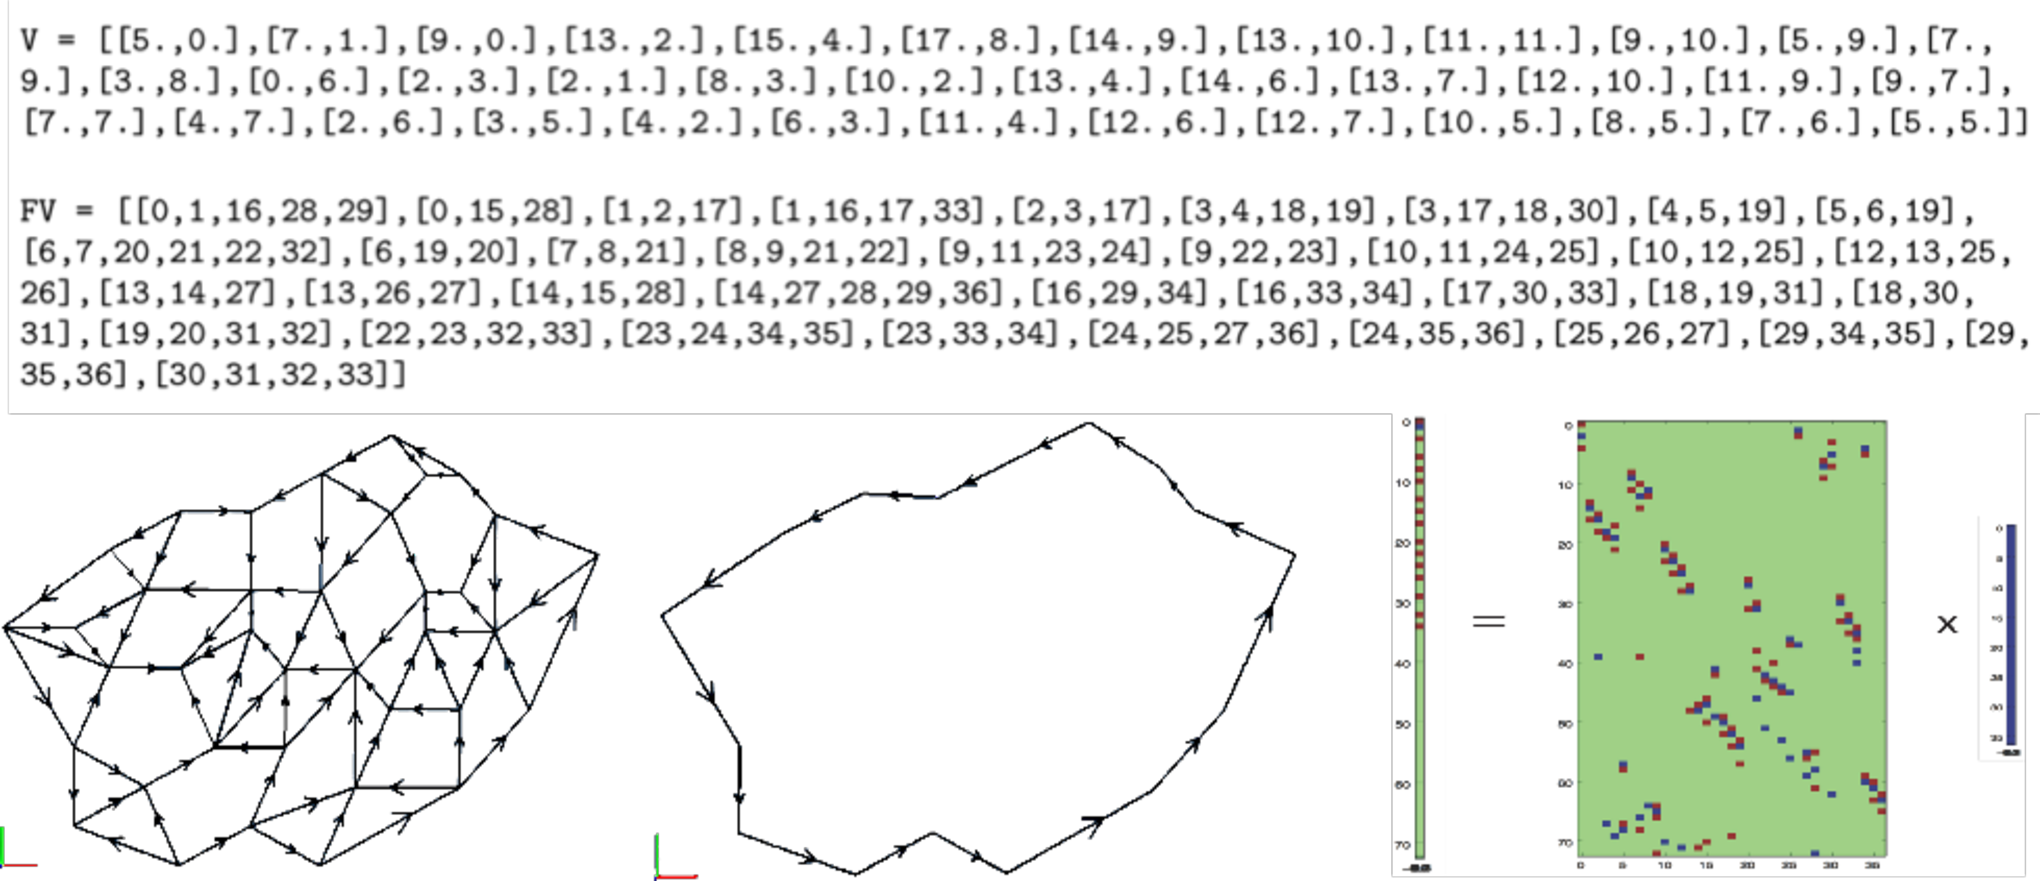
\includegraphics[width=\linewidth]{images/minimum} 
 \caption{A toy example of the LAR scheme: (a) the bare minimum of data with \emph{complete} information about topology; (b) the extracted boundary; (c) the extraction method $[e] = [\partial][f]$ giving the coordinate representation (in the discrete basis of the 1-cells) of the boundary edges $[e]$ by product of the sparse boundary operator matrix $[\partial]$ times the coordinate representation $[f]$ of the 2-cells (faces), in the discrete basis of the 2-cells.}
 \label{fig:minimum}
\end{figure}



\end{document}
